\chapter{Sécurité}

Ce chapitre a pour but d'examiner plus en détail les concepts de sécurité des protocoles qui peuvent être utilisés dans ce projet. 



\section{Bluetooth Low Energy}
\label{sec-security_ble}


Bluetooth est l'un des protocoles les plus utilisés pour réaliser des communications à courtes distances. Il implémente plusieurs mécanismes afin de chiffrer l'échange de données entre deux dispositifs.\\


\textbf{Note} : La section de ce rapport n'a pas pour objectif de traiter la cryptographie même du protocole Bluetooth, ni la manière dont les clés sont générées algorithmiquement. Pour des informations complémentaires sur la génération des clés, il est proposé de lire deux articles. Le premier est élaboré par l'instance officielle du Bluetooth et le deuxième est un \textit{whitepaper} rédigé par le très célèbre fabricant d'appareils de mesures électroniques Teledyne Lecroy : 
\begin{center}
    \footnotesize{\url{http://blog.bluetooth.com/bluetooth-pairing-part-1-pairing-feature-exchange}}
    \footnotesize{\url{http://www.fte.com/webhelp/sodera/Content/Documentation/WhitePapers/BTLE/BluetoothSmartSecurity.htm}}
\end{center}


La sécurité de la technologie Bluetooth a évolué au fil des diverses versions. Actuellement, les versions 4.2 et 5.0 ont les mêmes caractéristiques. Aucun élément de sécurité supplémentaire n'a été ajouté dans le Bluetooth 5.0 \cite{WhatsNe89:online}. Cependant, beaucoup de changements sont survenus entre les versions 4.0, 4.1 et 4.2. Ces anciennes versions ne seront pas abordées en détail, puisque presque aucun dispositif Bluetooth moderne n'est distribué sans le support de la version 4.2 au minimum. \\

Lors de l'explication des différents blocs de la couche \textit{Host} du Bluetooth, le bloc \texttt{Security Manager} a été abordé (cf. \cref{sec-protocols_BLE_security_manager}). Ce bloc s'occupe des générations et des sauvegardes de clés, de même que des méthodes et protocoles utilisés pour appairer deux dispositifs et partager les clés de connexion.\\

Lors de la mise en place d'une connexion sécurisée BLE, deux définitions sont utilisées :
\begin{itemize}
    \item Initiateur (\textit{initiator}) : correspond au maitre au niveau de la couche \texttt{Link Layer} et est aussi appelé centrale pour la couche GAP.
    \item Répondeur (\textit{responder}) : correspond à l'esclave au niveau de la couche \texttt{Link Layer} et est aussi appelé périphérique pour la couche GAP.
\end{itemize}

\subsection{Modes et niveaux de sécurité}
Dans la \cref{sec-protocols_BLE_GAP}, le bloc GAP a été défini comme étant l'élément s'occupant de l'authentification des centrales qui souhaitent se connecter auprès du périphérique. 
Il existe le concept de modes et niveaux de sécurité pour une connexion BLE. Voici la définition de ceux-ci :
\begin{enumerate}
    \item Mode 1 :
    \begin{enumerate}
        \item Niveau 1: Pas de sécurité (ni authentifiée, ni chiffrée);
        \item Niveau 2: Appairage non authentifié avec transfert de données chiffrées;
        \item Niveau 3: Appairage authentifié avec transfert de données chiffrées;
        \item Niveau 4: Appairage authentifié avec \textit{LE Secure Connections} et transfert de données chiffrées.
    \end{enumerate}
    \item Mode 2 :
    \begin{enumerate}
        \item Niveau 1: Appairage non authentifié avec transfert de données signées;
        \item Niveau 2: Appairage authentifié avec transfert de données signées.
    \end{enumerate}
\end{enumerate}


Toutes les connexions commencent en \textbf{mode 1} et \textbf{niveau 1} \cite{microchip_ble_security:online}. 

\subsection{Appairage et attachement}

L'appairage Bluetooth (\textit{pairing} en Anglais) est le processus qui définit l'échange des données de sécurité et la génération des clés \cite{BLEpairi85:online}\cite{Bluetoot72:online}.  Il y a au total trois phases lors de ce processus d'appairage, lesquelles sont visibles sur la \cref{fig-pairing-flowchart} et expliquées en détail dans les sous-sections qui suivent. 

\begin{figure}[ht!]
    \centering
    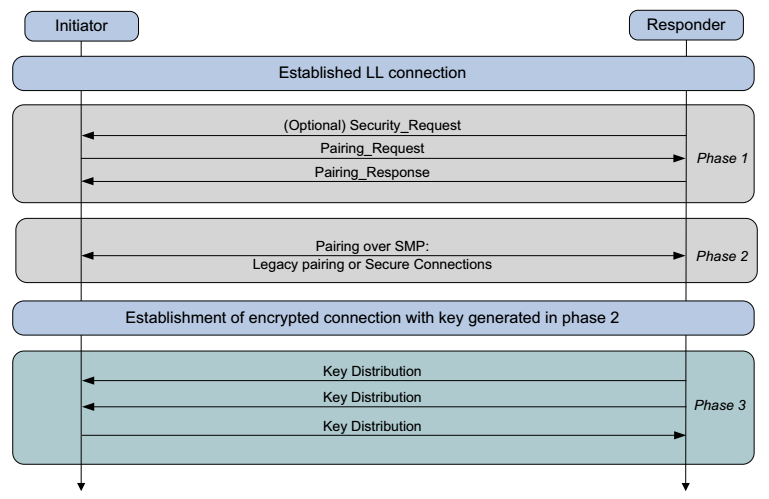
\includegraphics[width=1.0\textwidth]{Figures/Security/BLE/pairing-flowchart.png}
    \caption{Diagramme du processus d'appairage}
    \label{fig-pairing-flowchart}
\end{figure}

Ce processus de sécurité n'est pas forcément déclenché directement à la connexion, car plusieurs niveaux de sécurité peuvent être appliqués pour différents attributs. Par exemple, si une périphérique souhaite uniquement protéger un seul et unique attribut, il peut placer tous les autres attributs en Mode 1 Niveau 1. Le processus d'appairage ne sera déclenché que lorsque un attribut du mode 1 niveau 2 (au minimum) est accédé. L'appairage consiste à l'authentification de l'identité entre deux dispositifs et la création d'un canal chiffré utilisant une \textit{Short-Term Key} (STK). Une fois ce canal, créé, il faut ensuite distribuer des \textit{Long-Term Keys} (LTK), c'est à la fin de cette que la connexion est considéré comme attachée (\textit{bonded}). Les LTK seront ensuite sauvegardées sur les deux dispositifs pour chiffrer les futures communications sans nécessiter un nouvel appairage. \\

Il est important de comprendre le fonctionnement de ce processus, car tous ces modes doivent être configurés manuellement sur un microcontrôleur. 


\subsubsection{Phase 1: \textit{Pairing Feature Exchange}}

% TODO : 
% Cette phase a pour but d'échanger les informations sur les 
    
    
La phase 1 a pour objectif de partager les prérequis qui sont exigés pour la connexion.
Parmi ces données, on trouve diverses informations, telles que les entrées/sorties disponibles sur le périphérique, si l'utilisateur exige une protection \textit{man-in-the-middle} (MITM), etc. Ceux-ci seront ensuite analysés en phase 2 afin de s'assurer que le mode et niveau choisi pour la connexion est possible avec les informations fournies dans la phase 1. Les dispositifs doivent indiquer les capabilités de leurs I/O à l'aide des types définis sur la \cref{fig-io_capabilities} pour les entrées et \cref{fig-output_capabilities} pour les sorties.

\begin{figure}[ht!]
    \centering
    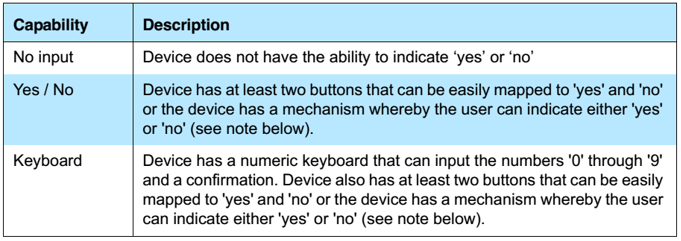
\includegraphics[width=0.85\textwidth]{Figures/Security/BLE/io_capabilities.png}
    \caption{Capacité des entrées disponibles sur un dispositif Bluetooth}
    \label{fig-io_capabilities}
\end{figure}

\begin{figure}[ht!]
    \centering
    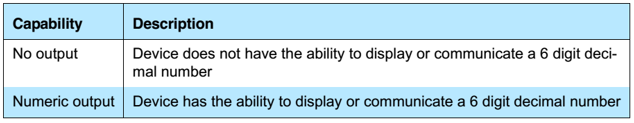
\includegraphics[width=0.85\textwidth]{Figures/Security/BLE/output_capabilities.png}
    \caption{Capacité des sorties disponibles sur un dispositif Bluetooth}
    \label{fig-output_capabilities}
\end{figure}



%OOB, or Out-of-Band, uses an external means of communication to exchange some information used in the pairing process. The OOB media could be any other wireless communication standard which can carry the corresponding information for pairing, like NFC or QRCode.

    
\subsubsection{Phase 2 : \textit{LE Legacy Pairing} ou \textit{LE Secure Connections}}


%After pairing feature exchange, initiator and responder should determine what key generation method will be used. Here is sample C syntax coding for the key generation method:

Après l'échange des \textit{pairing features} de la phase 1, la centrale et le périphérique doivent s'accorder sur quelle méthode utiliser pour l'échange et la génération des clés. \\



Depuis l'introduction du Bluetooth 4.2, si les deux dispositifs sont compatibles avec l'option LE Secure Connections et Secure Simple Pairing (SSP), alors il est conseillé d'utiliser ceux-ci (mode 1 niveau 4). La nouveauté majeure dans ce type de connexion est l'algorithme utilisé pour la génération des clés. Celui-ci est maintenant basé sur un échange et génération de clés publiques à l'aide de l'algorithme \textit{Elliptic Curve Diffie Hellman}\footnote{\url{https://en.wikipedia.org/wiki/Elliptic-curve_Diffie\%E2\%80\%93Hellman}} (ECDH) \cite{ble_basic_intro:online}. La \cref{fig-algorithms_4_2} illustre la différence entre le mode \textit{Legacy} (avant BLE 4.2) et les nouveaux algorithmes utilisés pour l'appairage et le \textit{bonding} \cite{Differen40:online}. \\


\begin{figure}[ht!]
    \centering
    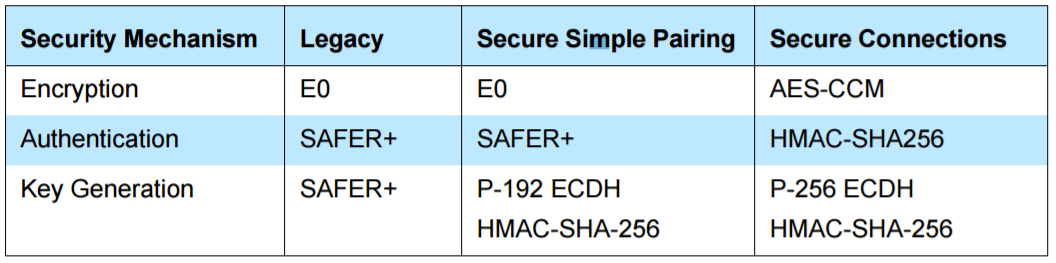
\includegraphics[width=0.85\textwidth]{Figures/Security/BLE/algorithms_4_2.PNG}
    \caption{Comparaison des algorithmes de générations de clés en fonction des versions BLE}
    \label{fig-algorithms_4_2}
\end{figure}



En Bluetooth Low Energy, il existe quatre méthodes pour la génération et l'échange de clés, de même que l'authentification de l'utilisateur: 

\begin{itemize}
    \item \texttt{\textit{\textbf{Just Works}}} : la STK est générée sur les deux dispositifs et est envoyée en \textit{plain-text}. Une fois ces clés publiques échangées, le \textit{responder} génère un \textit{nonce} aléatoire avec lequel il génère une valeur de confirmation nommée \texttt{Cb}. Ces deux paramètres (nonce et Cb) sont ensuite transmis à l'initiateur. En parallèle, l'initiateur génère son propre \textit{nonce} et le transfert au \textit{responder}. L'initiateur utilise ensuite le \textit{nonce} reçu de la part du \textit{responder} pour générer la valeur de confirmation nommée \texttt{Ca}. Les valeurs \texttt{Cb} et \texttt{Ca} doivent être identiques, si c'est le cas, la connexion est acceptée\cite{ble_basic_intro:online}.
    Cette méthode ne fournit pas d'opportunité à l'utilisateur de vérifier la légitimité du périphérique connecté. Une attaque de type \textit{man-in-the-middle} peut toujours prendre place\cite{microchip_ble_security:online}.
    
% The STK is generated on both sides, based on the packets exchanged in plain text. This method provides no security against man-in-the-middle (MITM) attacks.

% Once the devices exchange their public keys, the non-initiating device will generate a nonce, which is essentially a random seed value, and then use it to generate a confirmation value Cb. It then sends the Cb along with the nonce to the initiating device. At the same time, the initiating device generates its own nonce and sends it to the non-initiating device. The initiating device then uses the non-initiating device’s nonce to generate its own confirmation value Ca which should match Cb. If the confirmation values match, then the connection proceeds.

% By virtue of the ECDH key exchange, the Just WorksTM pairing method in LE Secure Connections has substantially more resilience to passive eavesdropping compared to the same method in LE Legacy Connections. However, since this method does not give the user a way to verify the authenticity of the connection, it is still vulnerable to MITM attacks.

    \item \texttt{\textit{\textbf{Passkey Display}}} : un des deux dispositifs affiche un code PIN (\textit{passkey}) de minimum 6 digits (en LE Secure Connection) et de préférence aléatoire. Le deuxième dispositif doit demander à l'utilisateur d'entrer le code affiché. Cette méthode Il faut donc au minimum un clavier sur un périphérique et un écran sur l'autre. Une protection \textit{man-in-the-middle} est prodigué, sauf si le PIN généré est à la vue de tous.
  
%   Passkey Display
% One of the peers displays a randomly generated 6-digit passkey and the other side as asked to enter it. In certain cases both sides enter the key, if no display is available. This method provides protection against MITM attacks.
    
    \item \texttt{\textit{\textbf{Out Of the Band (OOB)}}} : lors de la phase 1, les deux dispositifs indiquent s'ils acceptent un échange de clé par OOB. Cela signifie que l'échange de clés ne s'effectue pas à l'aide de la bande de fréquence du Bluetooth (2.4 GHz), mais à l'aide d'un autre mécanisme. Les méthodes les plus connues sont l'échange par communication NFC ou la lecture d'un QR code. \cite{microchip_ble_security:online} \cite{ble_basic_intro:online}.
    
%     Out of Band (OOB)
% This method has the additional data transferred by means other than the BLE radio (such as another wireless technology like NFC). This method also provides protection against MITM attacks.
    
    \item \texttt{\textit{\textbf{Numeric Comparison}}} : cette méthode utilise la même procédure que \texttt{Just Works}, mais rajoute une nouvelle étape à la fin. Une fois que les périphériques confirment la réception des \textit{nonces} utilisés pour la génération des clés, ils génèrent un nombre aléatoire avec ceux-ci. Les deux périphériques doivent ensuite l'afficher et si l'utilisateur voit que les deux valeurs sont identiques, alors il doit appuyer sur un bouton \textit{OK} pour valider que les deux périphériques soient bien authentifiés entre eux. Si ce n'est pas un cas, un bouton \textit{NOT OK} doit être pressé. \\
    
% Numeric Comparison (also called LE Secure Connections Pairing in BLE v4.2)
% This method uses an algorithm called Elliptic curve Diffie–Hellman (ECDH) for key generation, and a new pairing procedure for the key exchange.
% This pairing method follows the exact same procedure as the Just WorksTM pairing method, but adds another step at the end. Once the devices confirm that the confirmation values match, then both devices will independently generate a final 6 digit confirmation value using both of the nonces. They both then display their calculated values to the user. The user then manually checks that both values match and ok’s the connection. This extra step allows this pairing method to provide protection from MITM attacks.
\end{itemize}

Le choix de la méthode utilisée dépend ensuite des paramètres échangés à l'aide du \textit{pairing request} et \textit{pairing response}. Si l'option OOB est possible pour les deux périphériques, elle sera activée par défaut. Le reste des méthodes est choisi en fonction du tableau affiché sur la \cref{fig-ble_choose_security}. L'un des algorithmes présentés est ensuite choisi à la suite des paramètres échangé précédemment. \\


\begin{figure}[ht!]
    \centering
    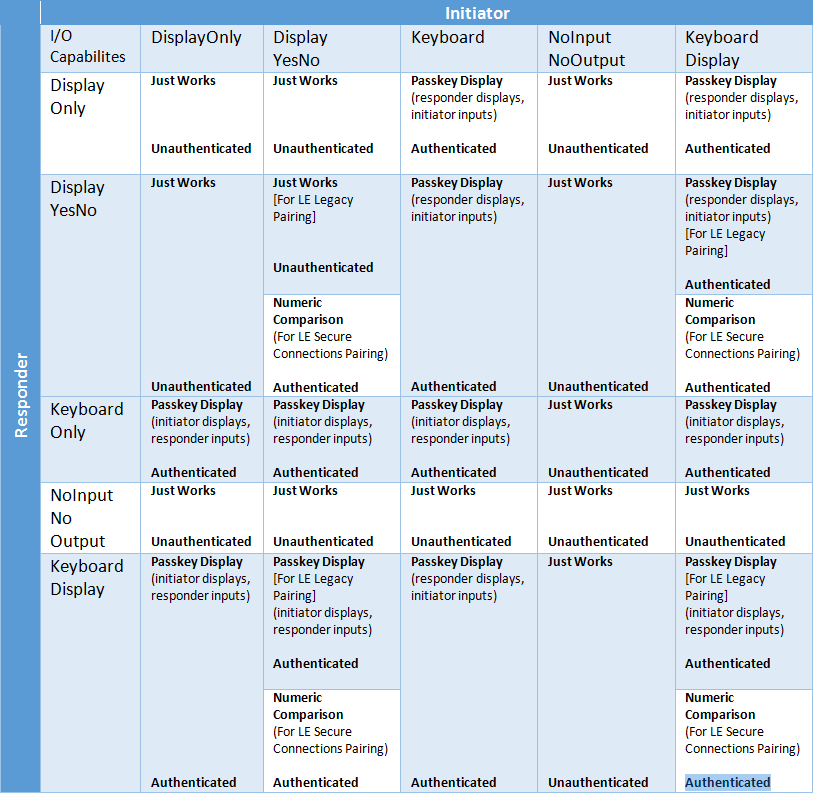
\includegraphics[width=1.0\textwidth]{Figures/Security/BLE/ble_choose_security.png}
    \caption{Choix de la méthode de sécurité en fonction des entrées/sorties}
    \label{fig-ble_choose_security}
\end{figure}

Dans le cas d'un smartphone, celui-ci dispose à la fois d'un clavier et d'un écran. Il offre donc le niveau de sécurité maximal pour l'échange d'informations à l'aide du Bluetooth. 
Le tableau de la \cref{fig-ble_choose_security} représente les recommandations pour les méthodes à utiliser, mais cela n'empêche pas le développeur de mettre en place, par exemple, un \textit{passkey} sans avoir d'écran sur le \textit{responder}. C'est l'une des raisons pour lesquelles beaucoup de périphériques dans le commerce utilisent des \textit{passkeys} tels que 0000 ou 1234 pour la première connexion. Pour cela, les périphériques sont obligés de mentir lorsqu'il envoie le paquet de réponses à l'initiateur. Ils indiquent qu'ils sont de type \textit{\textbf{display only}} alors que cette information est fausse. L'initiateur, la plupart du temps un smartphone ou ordinateur, choisi à l'aide du tableau la méthode qu'il doit appliqué et choisi \textit{initiator} : \textit{Keyboard} + \textit{Display} et \textit{responder} : \textit{display only}. Le smartphone demande ainsi à l'utilisateur d'enter le \textit{passkey}. 
Ce type d'approche détruit le concept d'authentification, car le but initial du \textit{passkey} est de s'assurer que la personne qui se connecte est bien celle qui est en face du périphérique, et donc qui a un accès physique à ce dernier avec la visibilité du \textit{passkey} sur l'écran. \\

Dans le cadre de ce projet, c'est le choix du \textit{passkey} qui a été retenu. Un \textit{passkey} aléatoire est présent dans chaque DevBox et est uniquement accessible à une personne de confiance (cf. \cref{sec-smartcanton_devbox_security} pour plus de détail sur l'implémentation). Mais le PIN n'est pas connu à l'avance, contrairement à la plupart des périphériques du marché où celui-ci est identique sur tous les périphériques vendus.\\




\subsubsection{Phase 3 : \textit{Transport Specific Key Distribution}}

Aussitôt que l'authentification est réussie, les deux dispositifs génèrent une Long Term Key (LTK) qui sera utilisée pour le chiffrement des futures connexions \cite{Bluetoot97:online}. Toutes les prochaines reconnexions des périphériques utiliseront cette clé, sans avoir besoin de réitérer les deux phases précédentes.




%-------------------------------------------------------------------------------------
\subsection{Recommandations de sécurité}
\label{sec-security_ble_recommendatiions}

En mai 2017, le National Institute of Standards and Technology (NIST) a publié un document intitulé \textit{Guide to Bluetooth Security}. Dans ce document de 67 pages, le NIST explique les vulnérabilités présentes sur des dispositifs Bluetooth, ainsi que les différentes failles qui peuvent y être associées \cite{GuidetoB8:online}. Le document analyse la sécurité de tous les protocoles Bluetooth récents (Low Energy ou \textit{Standard}). Il explique en outre les concepts de cryptographie qui sont utilisés pour la génération des clés. Voici le lien de la publication : 
\begin{center}
    \small{\url{http://nvlpubs.nist.gov/nistpubs/SpecialPublications/NIST.SP.800-121r2.pdf}}
\end{center}

À la fin dudit document, 37 recommandations sont proposées pour optimiser la sécurité sur un système utilisant le Bluetooth. Voici quatre exemples de recommandations extrêmement pertinentes pour le projet. La première indique le mode et le niveau de sécurité devant être utilisés sur les périphériques : 

\begin{quote}
\begin{center}
    \textit{"15. Bluetooth 4.2 devices and services using low energy functionality should use Security Mode 1 Level 4 whenever possible. Low energy Security Mode 1 Level 4 implements Secure Connections mode and provides the highest security available for 4.2 low energy devices. If Security Mode 1 Level 4 is not available, recommend using Security Mode 1 Level 3 instead"}
\end{center}
\end{quote}

Le KW41Z supporte tous les modes de sécurité et niveaux de sécurité. Cette recommandation peut ainsi être utilisée dans le projet.\\


Dans ce projet, un certain nombre de profils Bluetooth devant être implémentés, il est important de connaitre les recommandations y relatives. Voici la seule proposée pour les profils et services Bluetooth Low Energy dans le document : 

\begin{quote}
\begin{center}
    \textit{"17. Unneeded and unapproved service and profiles should be disabled. Many Bluetooth stacks are designed to support multiple profiles and associated services. The Bluetooth stack on a device should be locked down to ensure only required and approved profiles and services are available for use"}
\end{center}
\end{quote}

Par défaut, beaucoup de profils Bluetooth sont activés sur un même périphérique. Cependant, si l'utilisateur final n'a pas d'utilité à tous ces services, il convient de les désactiver afin qu'une éventuelle faille ne puisse être exploitée. Il est ici fait référence à des \textit{unapproved services}, référence qui peut être interprétée de deux façons. En premier lieu, il pourrait s'agir des services standards Bluetooth et fournis par la spécification Bluetooth. Néanmoins, cela semble beaucoup trop restrictif comme approche. Si un programmeur ne peut pas développer son propre service, il lui est impossible de faire certaines applications, car elles n'ont pas toutes été prévues par la spécification. L'on pourrait considérer, en second lieu, qu'aucun service non autorisé au sein du développement de l'application (par exemple un service de débogage) ne devrait être intégré dans le produit final. La seconde interprétation parait plus sensée avec les besoins des développeurs et des applications.\\

Lorsqu'une entreprise ou entité dispose de plusieurs périphériques Bluetooth Low Energy, il est important de garder une trace de ceux-ci, de sorte à créer une \textit{whitelist}. C'est pour cela que le NIST adresse la recommandation suivante :

 \begin{quote}
\begin{center}
    \textit{"6. Maintain a complete inventory of all Bluetooth-enabled wireless devices and addresses (BD\_ADDRs)."}
\end{center}
\end{quote}


Les dispositifs sont bien souvent protégés par des codes PIN, afin de ne pas autoriser n'importe quelle centrale à s'appairer avec celui-ci. NIST propose les recommandations suivantes pour la génération de ces codes PIN :
\begin{quote}
\begin{center}
    \textit{"9. Choose PIN codes that are sufficiently random, long and private. Avoid static and weak PINs, such as all zeroes. PIN codes should be random so that malicious users cannot easily guess them. Longer PIN codes are more resistant to brute force attacks. For Bluetooth 2.0 (or earlier) devices, an eight-character alphanumeric PIN should be used, if possible. The use of a fixed PIN is not acceptable."}
\end{center}
\end{quote}

Toutes ces recommandations sont parfois difficiles, voire impossibles à implémenter selon le type d'équipement utilisé. Si l'équipement le permet, il est toutefois préférable de les appliquer.




\newpage
\section{LoRaWAN}
\label{sec-security_lorawan}


La modulation LoRa en tant que telle ne comprend pas d'aspect lié à la sécurité, car il ne s'agit que de la couche 1 du modèle OSI. La sécurité est gérée par les couches supérieures, ce qui relève du protocole que l'utilisateur souhaite appliquer au-dessus de la modulation. Cette section sécurité se concentre principalement sur le mode OTAA pour l'enregistrement sur un réseau. Celui-ci est considéré comme étant le plus sûr et le mieux adapté à des dispositifs LoRaWAN \cite{ttnvideos_security:online}\cite{LoRaSecu3:online}.\\


Le 11 octobre 2017, la LoRa Alliance a dévoilé la version définitive du protocole LoRaWAN 1.1. Les explications prodiguées dans les sous-sections qui suivent décrivent la version 1.0.2 de LoRaWAN. Peu d'opérateurs proposent un support pour la spécification 1.1. Par exemple, le réseau The Things Network a pour objectif d'apporter un support uniquement pour avril ou mai 2018. Le module LoRaWAN choisi n'est actuellement pas encore compatible avec cette dernière version. Toutefois, la mise à jour des périphériques ne nécessite qu'une mise à niveau logicielle et non matérielle. Un résumé des nouveautés de LoRaWAN 1.1 est proposé en \cref{sec-security_lorawan_1_1}.\\


Le 23 mars 2016, la société MWR InfoSecurity\footnote{\url{https://www.mwrinfosecurity.com/}} spécialisée dans la recherche et les conseils en sécurité informatique a publié un \textit{whitepaper} sur la sécurité d'un réseau LoRa. Le document est intitulé \textit{LoRa Security: Building a secure LoRa solution} et écrit par Robert Miller \cite{LoRaSecu3:online}. Les explications du présent chapitre ont été en partie reprises de ce \textit{whitepaper}, lequel contient un résumé des points essentiels présentés dans la spécification LoRaWAN\footnote{\url{https://www.lora-alliance.org/lorawan-for-developers}}.


\subsection{Rejoindre un réseau à l'aide d'OTAA}
\label{sec-security_lorawan_join}


La structure des paquets LoRaWAN a été présentée en \cref{sec-protocols_lorawan}. Il est important d'avoir en tête les différents champs de ces paquets pour comprendre la façon dont la sécurité est appliquée aux messages LoRaWAN.

\begin{figure}[ht!]
    \centering
    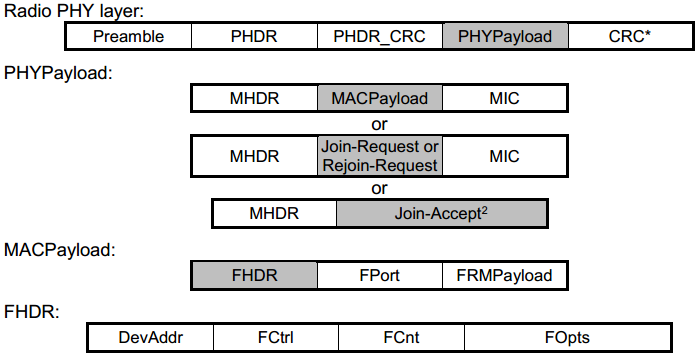
\includegraphics[width=0.8\textwidth]{Figures/Protocols/LoRaWAN/lorawan_mac_format_packets.png}
    \caption{Format des messages du protocole LoRaWAN}
    \label{fig-lorawan_mac_format_packets2}
\end{figure}

Chaque périphérique du réseau est déployé avec une \texttt{AppKey} et une \texttt{App EUI}. Cette première clé est indispensable lors de la procédure raccordement au réseau LoRaWAN pour authentifier le périphérique. L'\texttt{App EUI} est un identifiant qui est normalement unique pour l'utilisateur du périphérique et qui permet de déterminer à quelle application ce périphérique appartient. 
Pour initialiser cette procédure, le périphérique construit un message de type \texttt{Join Request} (cf. \cref{fig-lorawan_mac_format_packets2}) composé de l'\texttt{App EUI} de son \texttt{Dev EUI} de même que d'une valeur générée aléatoirement sur 2 bytes nommé DevNonce \cite{LoRaSecu3:online}. Le \texttt{Dev EUI} est l'identifiant unique du périphérique. Ces trois éléments sont ensuite signés à l'aide d'une valeur sur 4 bytes nommée \textit{Message Integrity Code} (MIC) et calculée comme suit :

\begin{tcolorbox}[top=-3mm, bottom=-3mm, left=0mm, right=0mm, enhanced, breakable, colback=LightGray, colframe=DarkGray, colbacktitle=DarkGray]
\begin{minted}[bgcolor=LightGray,fontsize=\footnotesize,breaklines]{python}
mac=aes128_cmac(AppKey, MHDR | AppEUI | DevEUI | DevNonce)
MIC = mac[0..3]
\end{minted}
\end{tcolorbox}


A la réception du message, le \textit{Network Server} détecte qu'il s'agit là d'un \textit{Join Request} et transfère la demande au \textit{Join Server} couplé à une valeur aléatoire (\textit{AppNonce}) qui sera utilisée pour la génération des clés. Le \textit{Join Server}vérifie les informations reçues afin de déterminer si le périphérique est ou non autorisé à rejoindre le réseau, puis il recalcule le MIC de son côté afin de s'assurer que le message n'a pas pu être altéré par une tierce personne. Si tout est validé, le \textit{Join Server} informe le \textit{Network Server} qu'une réponse de type \textit{Join Accept} doit être transmisse au périphérique. Cette réponse contient l'AppNonce précédemment généré par le \textit{Network Server}. Avec toutes ces informations, le serveur peut générer les deux clés de sessions (\textit{Network Session Key} et \textit{Application Session Key}) :

\begin{tcolorbox}[top=-3mm, bottom=-3mm, left=0mm, right=0mm, enhanced, breakable, colback=LightGray, colframe=DarkGray, colbacktitle=DarkGray]
\begin{minted}[bgcolor=LightGray,fontsize=\footnotesize,breaklines]{python}
NwkSKey = aes128_encrypt(AppKey, 0x01 | AppNonce | NetID | DevNonce | pad16)
AppSKey = aes128_encrypt(AppKey, 0x02 | AppNonce | NetID | DevNonce | pad16)
\end{minted}
\end{tcolorbox}

Le \textit{Join Accept} contient également les informations concernant les délais RF (RxDelay), le \textit{Dev Address} et la liste des canaux à utiliser (CFList). Un MIC doit être généré pour être ajouté au paquet de réponse :

\begin{tcolorbox}[top=-3mm, bottom=-3mm, left=0mm, right=0mm, enhanced, breakable, colback=LightGray, colframe=DarkGray, colbacktitle=DarkGray]
\begin{minted}[bgcolor=LightGray,fontsize=\footnotesize,breaklines]{python}
mac = aes128_cmac(AppKey, MHDR | AppNonce | NetID | DevAddr | RFU | RxDelay | CFList)
MIC = mac[0..3]
\end{minted}
\end{tcolorbox}

Les données sont retournées en utilisant l'\textit{AppKey} pour le chiffrement. A réception du paquet, le n\oe ud déchiffre les données et calcule à son tour les clés \textit{Network Session Key} et \textit{Application Session Key}. Ces deux clés sont maintenant utilisées pour chiffrer toutes les nouvelles données transmisses sur le réseau. La première pour les paquets qui sont envoyés sur le port 0 (\textit{Network Server}); la deuxième est quant à elle utilisée pour les données sur le port 1 à 223 impliquant l'\textit{Application Server}.

% La \cref{fig-keys_management_lorawan} démontre où les différentes clés de chiffrement sont présentes après qu'un périphérique aille rejoint un réseau en mode OTAA.

% \begin{figure}[ht!]
%     \centering
%     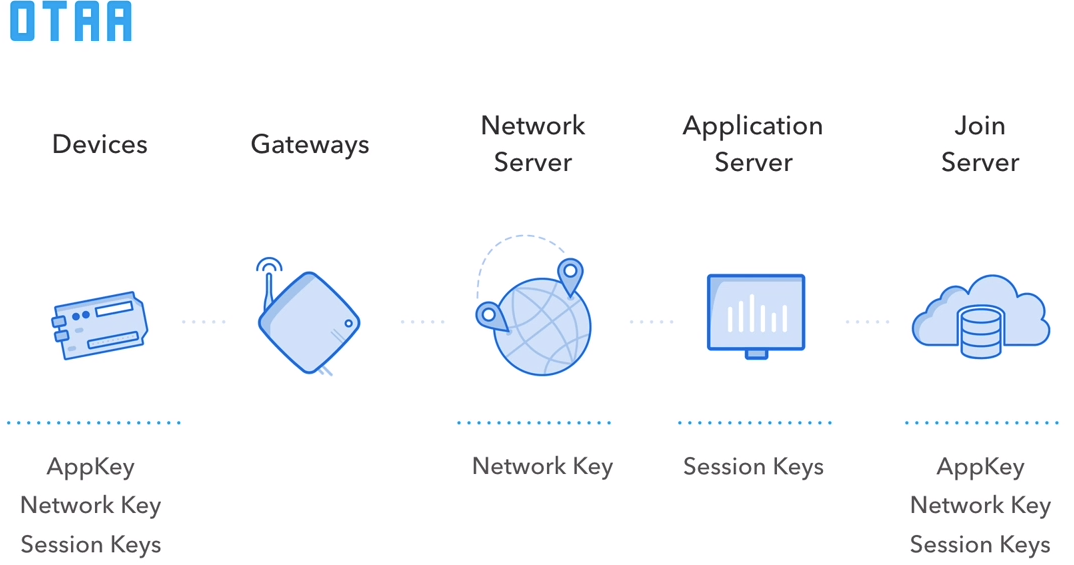
\includegraphics[width=0.8\textwidth]{Figures/Security/LoRaWAN/keys_management_lorawan.png}
%     \caption{Stockage des clés sur les différents composants d'une infrastructure LoRaWAN}
%     \label{fig-keys_management_lorawan}
% \end{figure}

\subsection{Protection des données}

Une fois un réseau LoRaWAN rejoint, toutes les données sont chiffrées en utilisant les deux clés de sessions.

\subsubsection{Chiffrement des données}

Le chiffrement des messages utilise AES-128\footnote{\url{https://en.wikipedia.org/wiki/Advanced_Encryption_Standard}} en \textit{Counter mode} (CTR) \cite{LoRaSecu3:online}. Une composante importante de la sécurité LoRaWAN réside dans les compteurs de messages \textit{uplink} (FCntUp) et \textit{downlink} (FCntDown) maintenus par le périphérique et le Network Serveur. Cette technique évite ainsi la possibilité de faire du \textit{replay attack}\footnote{\url{https://en.wikipedia.org/wiki/Replay_attack}} sur en copiant l'intégralité d'un paquet. 
Pour le chiffrement et le déchiffrement, un \textit{keystream} S est généré à l'aide des informations suivantes :

\begin{tcolorbox}[top=-3mm, bottom=-3mm, left=0mm, right=0mm, enhanced, breakable, colback=LightGray, colframe=DarkGray, colbacktitle=DarkGray]
\begin{minted}[bgcolor=LightGray,fontsize=\footnotesize,breaklines]{python}
i = 1..k where
k = ceil(len(FRMPayload) / 16)
Ai = (0x01 | (0x00 * 4) | Dir | DevAddr | FCntUp or FCntDown | 0x00 | i)
Si = aes128_encrypt(K,Ai), for i = 1..k
S = S1|S2|..|Sk
\end{minted}
\end{tcolorbox}

Une opération XOR est ensuite appliquée sur le champ \texttt{FRMPayload} avec le \textit{keystream} S pour chiffrer ou déchiffrer les données. Certaines données telles que le \texttt{FPort} ou \texttt{FCntUp} sont envoyées en clair.

\subsubsection{Signature des messages}

Dans le champ \textit{MAC Payload} (cf. \cref{fig-lorawan_mac_format_packets2}), les données sont singées afin d'éviter des modifications du \textit{cipher-text} ou d'autres valeurs comme le Dev Addr, FCnt ou FCntDown. De nouveau un champ MIC est utilisé comme signature :

\begin{tcolorbox}[top=-3mm, bottom=-3mm, left=0mm, right=0mm, enhanced, breakable, colback=LightGray, colframe=DarkGray, colbacktitle=DarkGray]
\begin{minted}[bgcolor=LightGray,fontsize=\footnotesize,breaklines]{python}
Msg = MHDR | FHDR | FPort | FRMPayload
B0 = (0x49 | 4*0x00 | Dir | DevAddr | FCntUp or FCntDown | 0x00 | len(msg) )
mac = aes128_cmac(NwkSKey, B0 | msg)
MIC = mac[0..3]
\end{minted}
\end{tcolorbox}


\subsubsection{Infrastructure des opérateurs LoRaWAN}
\label{sec-security_lorawan_providers}


L'architecture LoRaWAN a déjà été abordée en \cref{sec-protocols_lorawan_architecture}, avec la description des cinq composants principaux (périphérique, \textit{gateway}, \textit{Network Server}, \textit{Join Server} et \textit{Application Server}). \\
%Le stockage des clés sur les différents éléments du réseau est visible sur la \cref{fig-keys_management_lorawan}.\\

\begin{figure}[ht!]
    \centering
    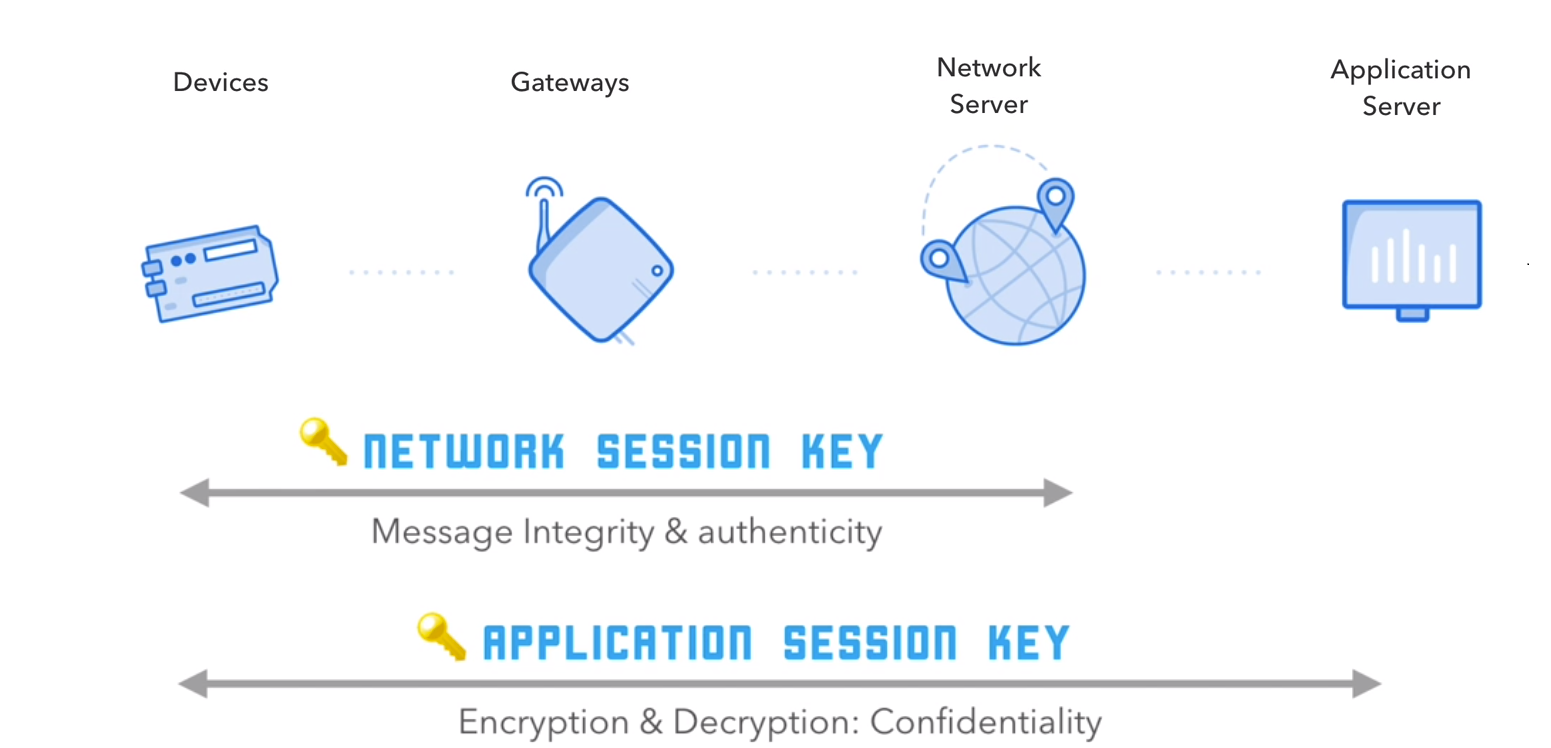
\includegraphics[width=0.85\textwidth]{Figures/Security/LoRaWAN/by_design_keys.PNG}
    \caption{Infrastructure d'un réseau LoRaWAN comme imaginée dans la spécification}
    \label{fig-by_design_keys}
\end{figure}

Le schéma de la \cref{fig-by_design_keys} expose l'utilisation des clés dans un réseau LoRaWAN. L'infrastructure y étant illustrée affiche une configuration pensée dans la spécification LoRaWAN: une séparation entre le \textit{Network Server} et l'\textit{Application Server}. \\

La réalité est quelque peu différente de cette implémentation. En effet, la plupart des fournisseurs de réseau LoRaWAN (The Things Network, Swisscom, Loriot, etc.) n'offrent pas la possibilité de séparer ces deux entités. L'architecture pratiquée par ces opérateurs est visible sur la \cref{fig-in_practice_keys}. L'opérateur possède les deux serveurs et fournit un accès au données au travers d'API propres à chacun. Cette architecture présente une problématique pour la sécurité des données. En effet, l'opérateur a à sa disposition la clé la plus importante, l'AppKey. Avec celle-ci, il doit générer la Network Session Key, indispensable à l'opérateur, et l'Application Session Key pour déchiffrer les données fournies à l'utilisateur. 
La plupart des opérateurs ont choisi cette approche puisque les clients ne souhaitent pas nécessairement mettre en place un \textit{Application Server} et un \textit{Join Server} en interne. Le SmartCanton a quant à lui décidé d'utiliser cette approche afin de garantir une sécurité et une maitrise totale sur les données tout en utilisant les infrastructures d'un opérateur existant pour le transport des paquets (cf. \cref{sec-smartcanton_security}).


\begin{figure}[ht!]
    \centering
    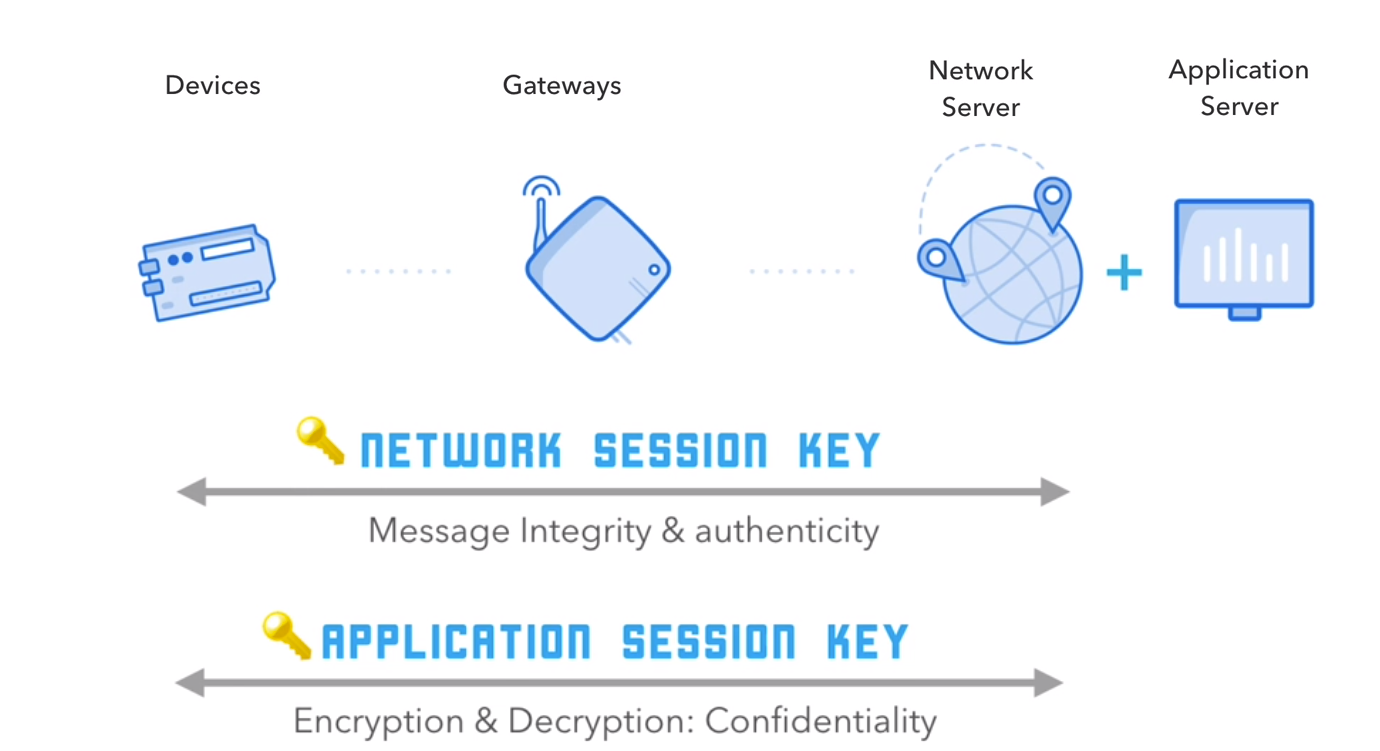
\includegraphics[width=0.85\textwidth]{Figures/Security/LoRaWAN/in_practice_keys.PNG}
    \caption{Infrastructure d'un réseau LoRaWAN réellement implémenté avec les opérateurs du marché}
    \label{fig-in_practice_keys}
\end{figure}



% ---------------------------------------------------------------------------------------
\subsection{LoRaWAN spécification 1.1}
\label{sec-security_lorawan_1_1}
% ---------------------------------------------------------------------------------------

La spécification LoRaWAN 1.1 apporte de nouvelles améliorations dans le domaine de la sécurité avec l'ajout de nouveaux concepts et des changements de mécanismes \cite{lorawan1_1_video:online}. Voici un résumé des changements principaux :
\begin{itemize}
    \item le compteur du nombre de paquets envoyés doit être stocké dans une mémoire non volatile et le même compteur ne peut pas être utilisable dans une même session. Un périphérique ABP ne peut ainsi plus être remis à zéro;
    
    \item DevNonce et JoinNonce (précédemment nommé AppNonce) ne sont plus aléatoire. Ce sont maintenant des valeurs incrémentales qui ne peuvent être utilisées qu'une seule fois et doivent être stockées en mémoire non volatile sur le périphérique;
    
    \item compteurs de message sur 32 bits (il s'agissait précédemment d'une recommandation, la version 16 bits était autorisée);
    
    \item deux compteurs de messages \textit{downlink} séparés; un pour le réseau (NFCntDown), l'autre pour l'application (AFCntDown);
    
    \item le compteur d'\textit{uplink} (FCntUp) est maintenant utilisé pour générer le MIC de l'\textit{acknowledge}.
    
\end{itemize}

Tous les périphériques doivent obligatoirement avoir la possibilité de stocker en mémoire non volatile les différentes informations. C'est la seule obligation matérielle impérative sur les périphériques 1.1. 

\begin{figure}[ht!]
    \centering
    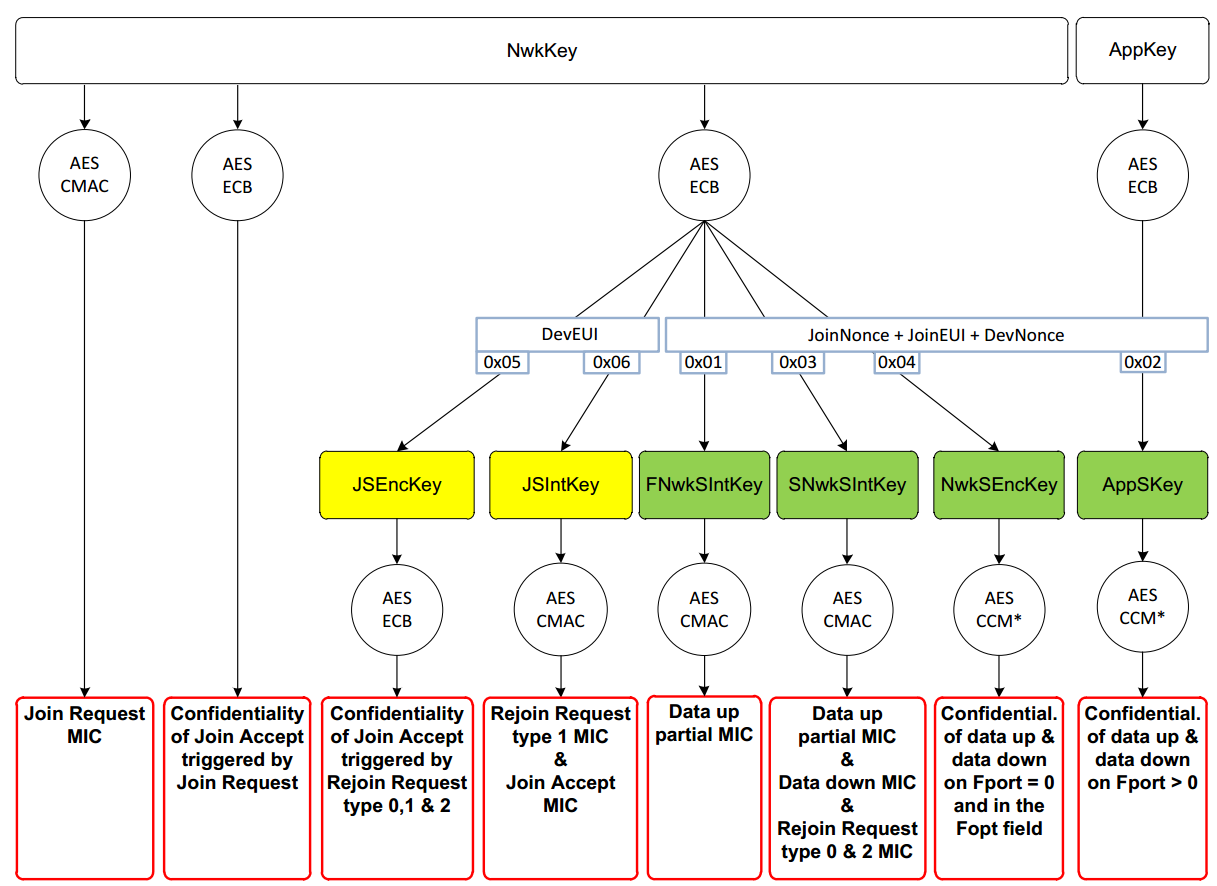
\includegraphics[width=1.0\textwidth]{Figures/Security/LoRaWAN/lorawan1_1_keys.PNG}
    \caption{Clés utilisées dans un réseau LoRaWAN avec la nouvelle spécification 1.1}
    \label{fig-lorawan1_1_keys}
\end{figure}

Le changement le plus important de la spécification 1.1 est l'introduction d'un nouveau secret partagé, nommé Network Key (\textbf{NwkKey}). Cette clé est utilisée pour créer trois nouvelles clés : 
\begin{enumerate}
    \item NwkSEncKey : clé utilisée pour chiffrer les commandes MAC;
    \item SNwkSIntKey : utilisée par un \textit{Serving Network Server} pour le calcul de la première moitié du MIC;
    \item FNwkSIntKey : utilisée par le \textit{Forwarding Network Server} pour le calcul de l'autre moitié du MIC.
\end{enumerate}

Une meilleure vue d'ensemble de toutes les clés et leur utilité est visible à l'aide de la \cref{fig-lorawan1_1_keys}. Si un périphérique 1.1 souhaite rejoindre un réseau gouverné par un Network Serveur 1.0, toutes les clés seront calculées à l'aide de la NwkKey. Les clés de sessions seront identiques et le périphérique n'utilisera plus sa AppKey. \\


Conjointement avec la parution de la spécification LoRaWAN 1.1, une nouvelle spécification pour la \textit{backend} des réseaux LoRaWAN nommée \textit{LoRaWAN Backend Interfaces 1.0 Specification} est disponible \cite{loraalli46:online}. Les informations de celles-ci affectent principalement les opérateurs de réseau LoRaWAN.

% ---------------------------------------------------------------------------------------
\subsection{Vulnérabilités et recommandations de sécurité}
\label{sec-security_lorawan_recommendatiions}
% ---------------------------------------------------------------------------------------

Les sous-sections qui suivent proposent quelques recommandations aux vulnérabilités sur les réseaux LoRaWAN \cite{ttnvideos_security:online} \cite{LoRaSecu3:online}. La spécification 1.1 apporte de nouvelles améliorations, toutefois certaines recommandations restent d'actualités \cite{lorawan1_1_video:online}.  

\subsubsection{Infrastructure du réseau}

L'infrastructure des opérateurs d'un réseau LoRaWAN a été étudiée en \cref{sec-security_lorawan_providers}. Laquelle a permis d'exposer la problématique sur le contrôle des serveurs. La plupart des opérateurs offrent une infrastructure complète avec l'intégration des trois serveurs. Il existe deux solutions pour pallier à cette problématique : 
\begin{enumerate}
    \item Utiliser un opérateur autorisant la connexion avec un \textit{Join Server} et un \textit{Application Server} externe. Cette approche est visible sur la \cref{fig-recommendations_a_private_domain}. Il s'agit là d'une réelle séparation des données et du réseau, comme la spécification LoRaWAN l'a prévu.
    
\begin{figure}[ht!]
    \centering
    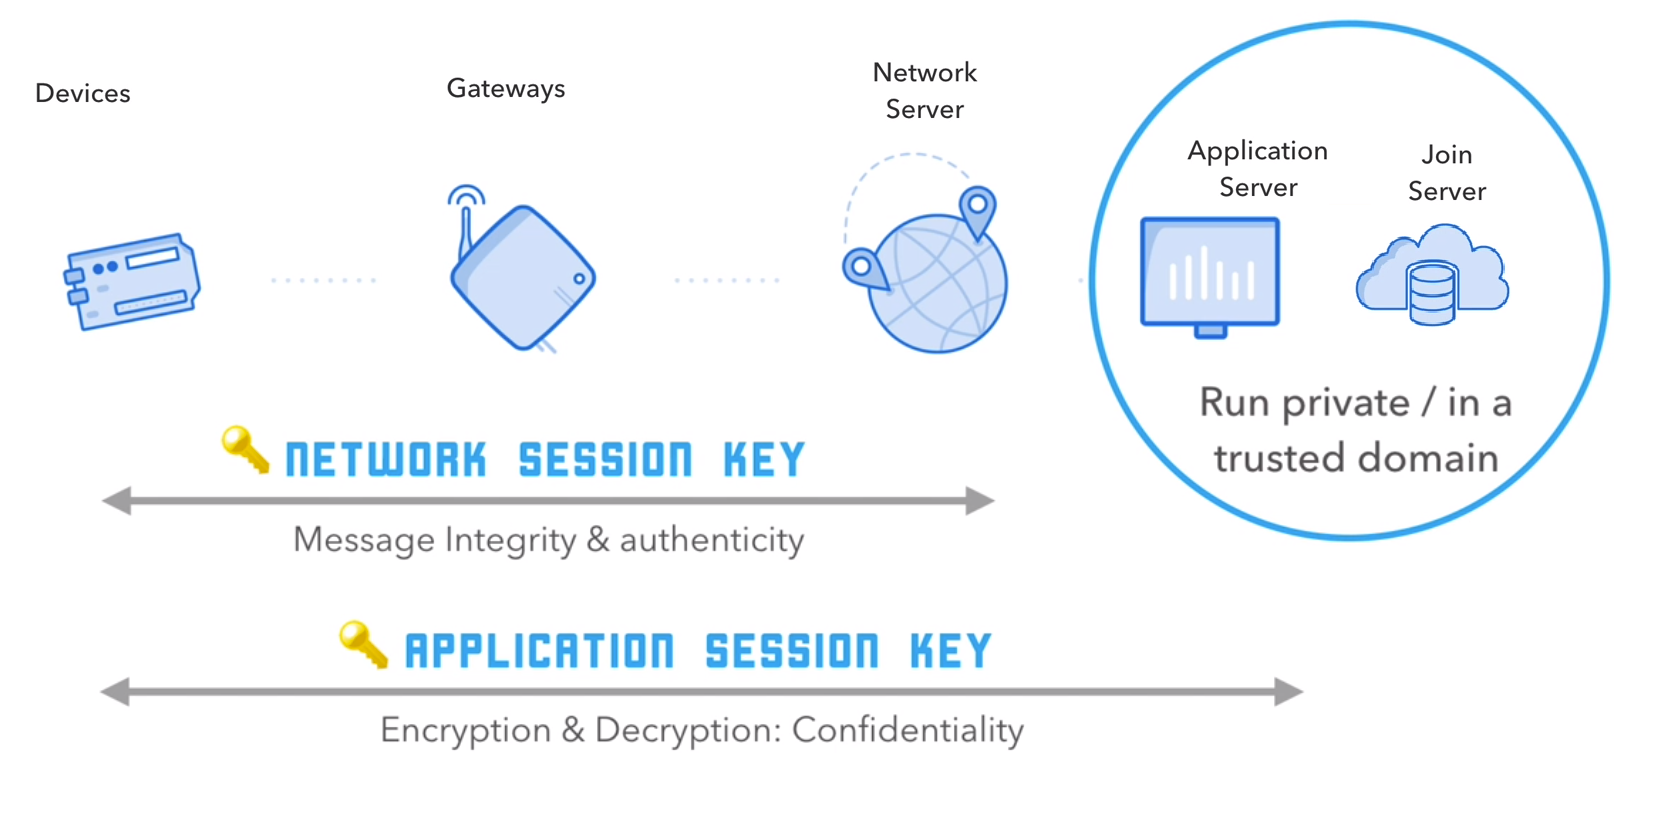
\includegraphics[width=0.9\textwidth]{Figures/Security/LoRaWAN/recommendations_a_private_domain.PNG}
    \caption{Recommandation pour l'implémentation d'une infrastructure LoRaWAN sécurisée}
    \label{fig-recommendations_a_private_domain}
\end{figure}

    \item Ajouter une nouvelle étape de chiffrement asymétrique, exploré sur la \cref{fig-recommendations_b_asymetric_crypto}. Lorsque cette option est utilisée, un opérateur de réseau LoRaWAN ne peut pas déchiffrer. Le déchiffrement peut ensuite être effectué par l'application finale qui se connecte au flux provenant de l'\textit{Application Server}.
    
\end{enumerate}




\begin{figure}[ht!]
    \centering
    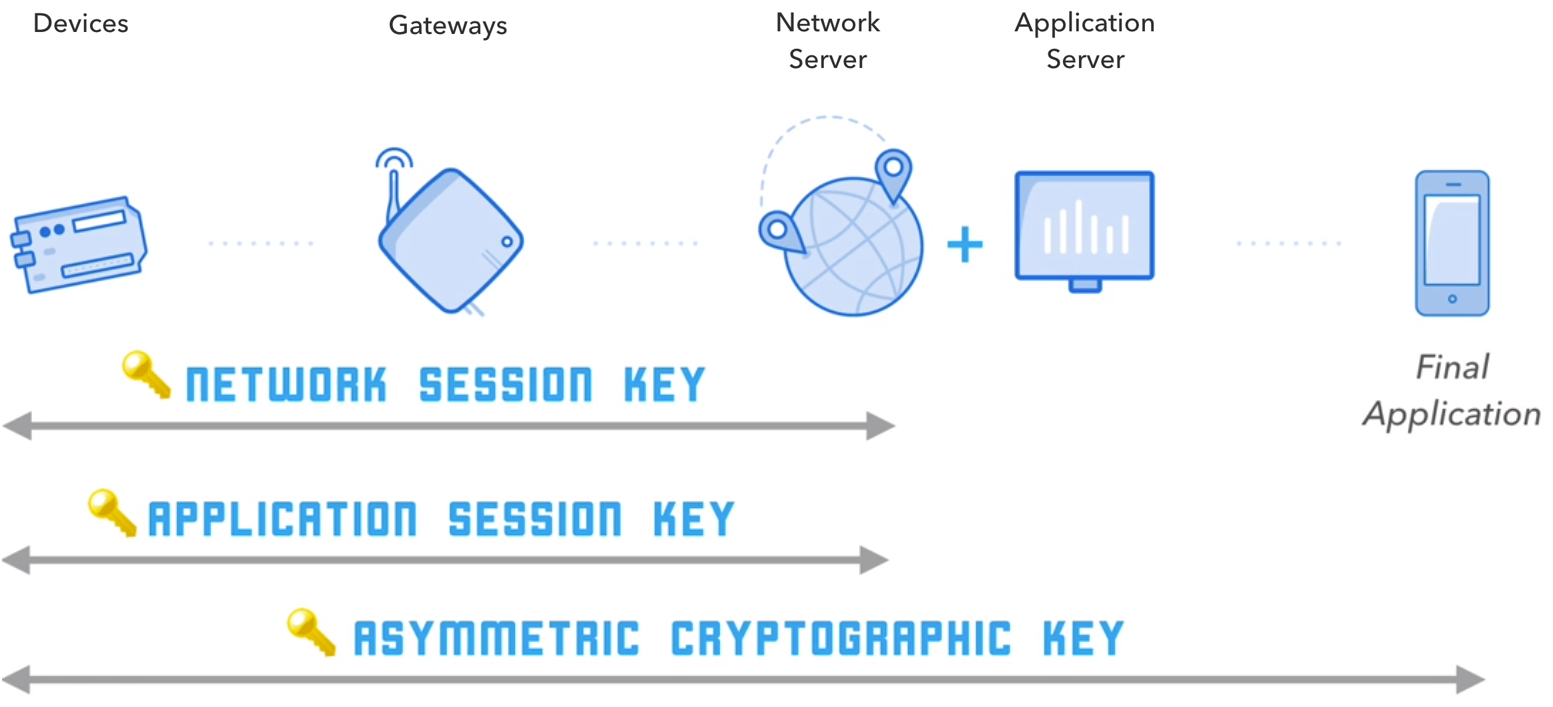
\includegraphics[width=0.9\textwidth]{Figures/Security/LoRaWAN/recommendations_b_asymetric_crypto.png}
    \caption{Clé asymétrique utilisée pour chiffrer les données}
    \label{fig-recommendations_b_asymetric_crypto}
\end{figure}


\subsubsection{Gestion des clés pour les périphériques}


Le mode de connexion le plus sécurisé est l'OTAA, car il ne nécessite que la connaissance d'un seul et unique secret partagé entre le \textit{Join Server} et le périphérique, l'AppKey. Lorsque l'une des deux clés de sessions est compromise, le périphérique peut être forcé à se joindre à nouveau au réseau et ainsi régénéré de nouvelles clés de session. La programmation des clés en ABP n'offre pas cette possibilité.\\

Un attaquant peut toujours récupérer des clés de chiffrements lorsqu'un accès direct au périphérique est possible. Par exemple, les attaques de type \textit{side channel analysis} qui consistent à mesurer la variation de courant ou la mesure des radiations électromagnétiques lorsque le \textit{transceiver} effectue le chiffrement AES pour déterminer la clé utilisée \cite{LoRaSecu3:online}. \\

Toutes les clés stockées sur les périphériques doivent être uniques. Il est possible d'assigner la même AppKey pour tous les périphériques, puisque l'identifiant unique du périphérique est le Dev EUI. Toutefois, ceci ne devrait jamais être le cas, car il suffit qu'un seul périphérique soit compromis pour que tous les périphériques d'un réseau doivent être reprogrammés. \\

La programmation des clés sur les périphériques ne doit pas se faire à l'aide de la même plage de fréquence que le LoRa \cite{ttnvideos_security:online}. Il est conseillé d'utiliser un nouveau type accès et ainsi appliquer un concept de \textit{out of the band}\footnote{\url{https://en.wikipedia.org/wiki/Out-of-band_data}} pour l'authentification, par exemple, en utilisant une technologie en 2.4 GHz. \\

Il est parfois possible d'envoyer un fichier binaire aux fabricants de cartes électroniques pour qu'ils programment directement les microcontrôleurs à la suite du montage des cartes électroniques \cite{ttnvideos_security:online}. Cette méthode est fortement déconseillée si le fabricant n'est pas de confiance. \\
 
Les clés ne doivent pas être stockées en tant que constantes dans le \textit{firmware} du microcontrôleur et la mémoire du microcontrôleur doit être sécurisée (cf. \cref{sec-security_hardware_protections} pour plus d'informations).


\subsubsection{Gestion des clés pour les serveurs}


Les serveurs doivent avoir accès aux différentes clés afin d'effectuer leurs tâches, mais celles-ci ne doivent être accessibles qu'à des personnes autorisées, que ce soit en lecture ou en écriture. \\

La génération de ces clés (cf. \cref{sec-security_lorawan_join}) doit être aléatoire, par exemple, en utilisant des \textit{true random number generators}.


\subsubsection{Compteur de paquets}

La vérification des compteurs de paquets doit être correctement effectuée par le \textit{Network Server}. Certains opérateurs allouent à l'utilisateur la possibilité de désactiver cette option pour effectuer des tests, mais ceci n'est pas acceptable lors d'une implémentation définitive. 


\subsubsection{Renouvellement des clés OTAA}


Lorsqu'un périphérique rejoint un réseau en OTAA, les clés de sessions générées sont utilisables indéfiniment \cite{ttnvideos_security:online}. Si le périphérique accepte les \textit{uplinks}, une commande applicative peut être envoyée pour demander au périphérique de relancer une nouvelle session à l'aide d'un \textit{join request}. Si les paquets \textit{downlink} ne sont pas implémentés, cette procédure peut être automatisée en local après l'envoi d'un nombre défini de paquets \textit{uplink}. Cette problématique a été corrigée avec le LoRaWAN 1.1 avec l'ajout de nouvelles commandes pour forcer un \textit{rejoin} du réseau en OTAA.


\subsubsection{Usurpation du microcontrôleur}




\begin{figure}[ht!]
    \centering
    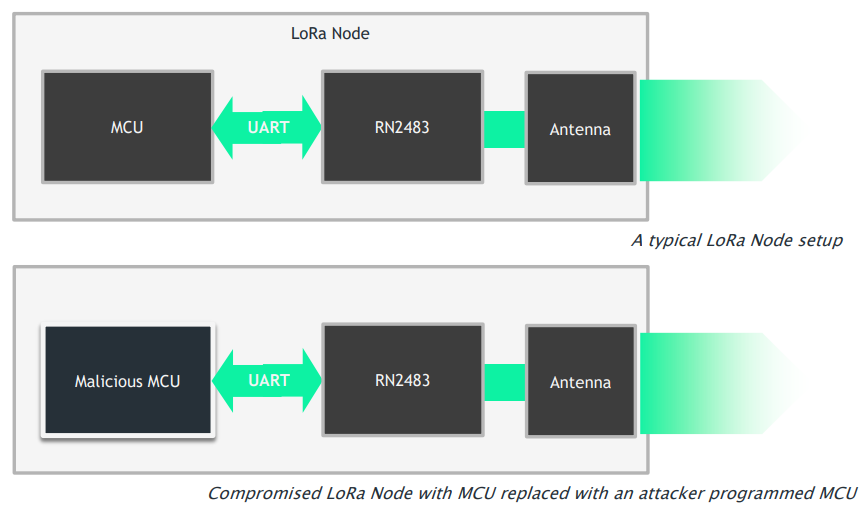
\includegraphics[width=0.65\textwidth]{Figures/Security/LoRaWAN/hardware_attack.png}
    \caption{Vulnérabilité des modules LoRaWAN avec le remplacement du microcontrôleur}
    \label{fig-hardware_attack}
\end{figure}

Lorsque l'attaquant dispose d'un accès direct sur le matériel, il lui est possible d'usurper le microcontrôleur principal communiquant. Par exemple, le RN2483 de Microchip \footnote{\url{https://www.microchip.com/wwwproducts/en/RN2483}} offre une interface UART pour la configuration. La \cref{fig-hardware_attack} expose la situation. Une solution pour pallier à ce type d'attaque consiste à utiliser un module qui ne peut pas être lu depuis l'extérieur. Une fois celui-ci programmé pour rejoindre un réseau, il sauvegarde dans sa mémoire non volatile les clés sans les redistribuer.
Il est possible de ne pas utiliser de coprocesseur LoRaWAN et d'implémenter la \textit{stack} LoRaWAN directement dans le processeur principal. On peut ainsi utiliser un circuit intégré radio de Semtech. Les inconvénients de ce type d'implémentation est la complexité logicielle ajoutée au processeur principal. En \cref{sec-security_hardware_protections} divers conseils relatifs au stockage des clés dans des mémoires non volatiles sont présentés.


\subsubsection{Accès aux \textit{gateways}}

Si un attaquant a accès à une \textit{gateway}, il ne peut pas accéder aux données, car celles-ci sont toujours chiffrées avec les différentes clés. Toutefois, il a la possibilité de la rendre inopérationnelle. L'attaquant peut également corrompre les données, mais dans ce cas, le \textit{Network Server} détectera cette corruption et les ignorera.
Les \textit{gateways} sont le plus souvent connectées à Internet pour créer le pont entre le protocole LoRaWAN et les serveurs. Il est important de les mettre à jour régulièrement, et tout particulièrement lorsqu’une vulnérabilité est découverte ou lorsqu'une nouvelle version du protocole est disponible. Cette mise à jour peut se faire en se déplaçant physiquement auprès de celle-ci ou à distance. La deuxième option est indispensable lorsqu'un grand parc de \textit{gateways} est maintenu. La connexion à celle-ci doit donc être sécurisée du mieux possible à l'aide mots de passe uniques pour chaque \textit{gateway} ou encore mieux, des clés d'authentifications (ex. clés SSH) gardées secrètes. 



\subsection{SmartCanton}
\label{sec-smartcanton_security}



Le POC SmartCanton a été présenté brièvement en \cref{sec-stateoftheart_smartcanton}. Il en est ressorti la forte sécurité qui a été implémentée et pensée dans ce projet.
À la \cref{sec-security_lorawan}, la sécurité LoRaWAN a été étudiée de façon générale. En fin de la \cref{sec-security_lorawan}, des recommandations pour des réseaux et périphériques LoRaWAN ont été présentées. Le POC SmartCanton a pris très au sérieux les problématiques liées à la sécurité dans l'implémentation du projet. Les buts des sous-sections qui suivent sont d'explorer quels mécanismes ont été appliqués et ainsi mieux comprendre l'intérêt de la mise en place de ce travail de Master.


\subsubsection{\textit{Hardware Security Module}}

Le SmartCanton s'est équipé d'un Hardware Security Module (HSM) de la série Nshield\footnote{\url{https://www.thalesesecurity.com/products/general-purpose-hsms/nshield-connect}} de l'entreprise Thales. Ce composant est utilisé pour générer les clés, mais également pour les stocker. Il s'agit là d'un coffre-fort inviolable et hautement certifié. Une donnée chiffrée peut lui être envoyée pour être déchiffrée, comme l'exemple avec le \textit{Join Server} sur la \cref{fig-nshield_thales}.

\begin{figure}[ht!]
    \centering
    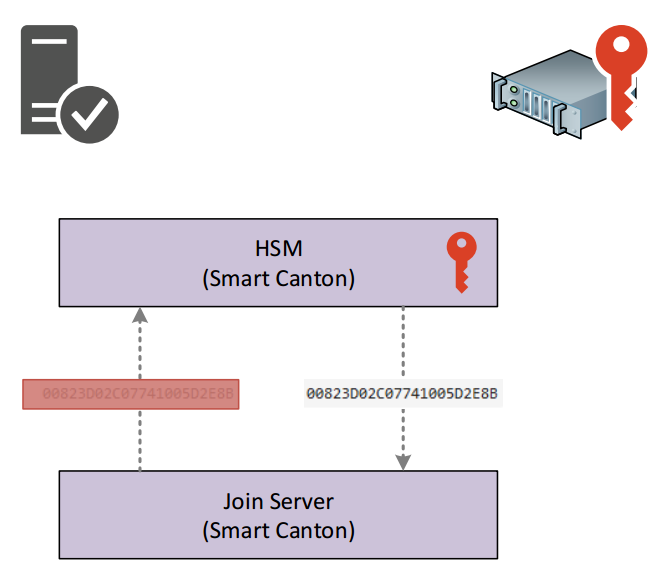
\includegraphics[width=0.5\textwidth]{Figures/Security/smartcanton/nshield_thales.png}
    \caption{Thales Nshield}
    \label{fig-nshield_thales}
\end{figure}



\subsubsection{\textit{Join Server}}

Pour faciliter la lecture des diagrammes du SmartCanton qui suivent, voici la légende des couleurs des clés utilisées : 
\begin{itemize}
    \item \textcolor[rgb]{0,0,1}{\textbf{Bleu}} : Application Key (AppKey);
    \item \textcolor[rgb]{1,0,0}{\textbf{Rouge}} : Application Session Key (AppSKey);
    \item \textcolor[rgb]{1,0.8,0}{\textbf{Orange}} : Network Session Key (NwkSKey).\\
\end{itemize}

\begin{figure}[ht!]
    \centering
    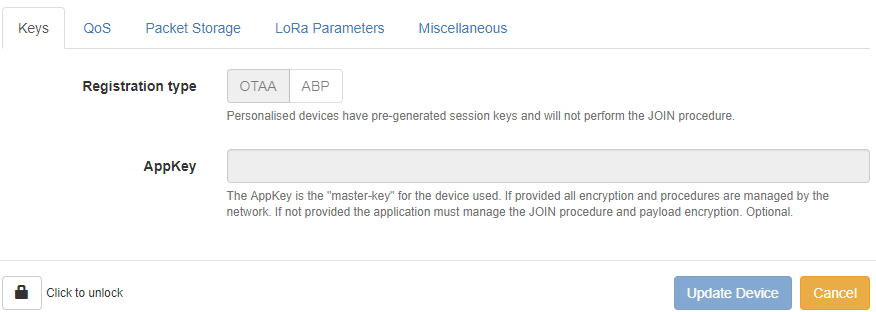
\includegraphics[width=0.55\textwidth]{Figures/Security/smartcanton/orbiwise_no_appkey.png}
    \caption{Périphérique enregistré sur un réseau OrbiWise sans AppKey}
    \label{fig-orbiwise_no_appkey}
\end{figure}

La fédération des opérateurs implémentée dans le POC est présentée à la \cref{fig-federation_network}, celle-ci est une composante primordiale pour la couverture en réseau du canton et de la ville de Genève. Le réseau d'OrbiWise autorise la création d'un périphérique sans spécification d'AppKey (cf. \cref{fig-orbiwise_no_appkey}, contrairement à TTN et Swisscom où cela est impossible. Cette fédération nécessite la redirection des requêtes vers un \textit{Join Server} personnalisé. Ce \textit{Join Server} est directement connecté au HSM pour la gestion des clés (cf. \cref{fig-nshield_thales}).\\


\begin{figure}[ht!]
    \centering
    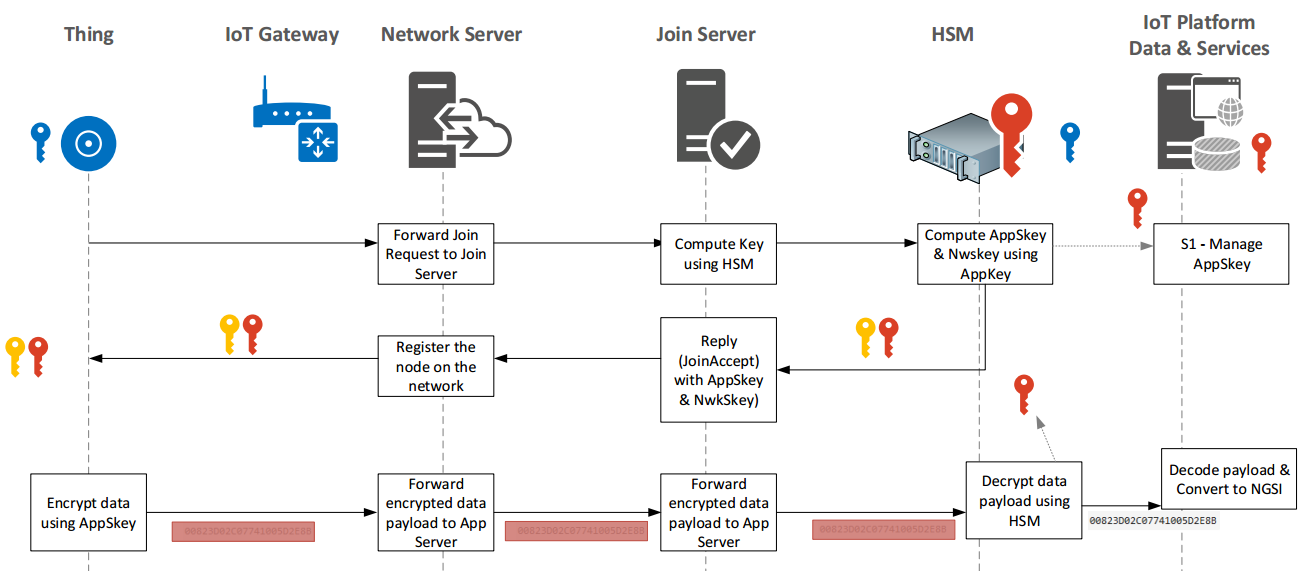
\includegraphics[width=1.0\textwidth]{Figures/Security/smartcanton/smartcanton_joinserver_decrypt_hsm.png}
    \caption{Déchiffrement des données par le HSM}
    \label{fig-smartcanton_joinserver_decrypt_hsm}
\end{figure}


OrbiWise équipe son infrastructure d'origine avec deux composants: un \textit{Network Server} (NST) pour la gestion du réseau et un Data Access Sub-System (DASS) qui équivaut à un \textit{Application Server} pour la récupération des données. Le \textit{Join Server} du SmartCanton travaille en tandem avec le Network Server d'OrbiWise pour récupérer les paquets qui sont envoyés par des périphériques inconnus au réseau d'OrbiWise. La \cref{fig-smartcanton_joinserver_decrypt_hsm} décrit la séquence complète de connexion d'un nouveau périphérique sur le réseau. Voici les points clés à retenir lors de la séquence de connexion à un partenaire du POC SmartCanton : 
\begin{enumerate}
    \item Le périphérique envoie un \textit{Join Request} sur le réseau.
    \item La \textit{gateway} de l'opérateur partenaire le récupère et l'envoi au \textit{Network Server} de l'opérateur.
    \item Le \textit{Network Server}, génère un AppNonce et l'envoi, conjointement à la demande de \textit{Join Request}, au \textit{Join Server} du SmartCanton.
    \item Le \textit{Join Server} identifie le périphérique comme étant autorisé à rejoindre le réseau et demande au HSM de créer les clés de sessions pour ce dernier. Une copie des clés est conservée à l'intérieur du HSM.
    \item Le Join Server construit et chiffre le Join Accept et le renvoi au Network Server accompagné de la NwkSKey.
    \item Le \textit{Network Server} \textit{forward} le \textit{Join Accept} vers le périphérique et sauvegarde en local la NwkSKey pour les futures communications avec le périphérique.
\end{enumerate}


\subsubsection{Cheminement des données et répartition des clés}

Le POC SmartCanton a pensé à deux implémentations de déchiffrement en utilisant les clés : 
\begin{enumerate}
    \item le déchiffrement des données est géré directement par le HSM. Cette implémentation est celle visible sur la \cref{fig-smartcanton_joinserver_decrypt_hsm}.
    \item le déchiffrement des données est géré par la plateforme IoT, par exemple, dans un module FIWARE. Cette implémentation est quant à elle visible sur la \cref{fig-smartcanton_joinserver_decrypt_hsm}.
\end{enumerate}

\begin{figure}[ht!]
    \centering
    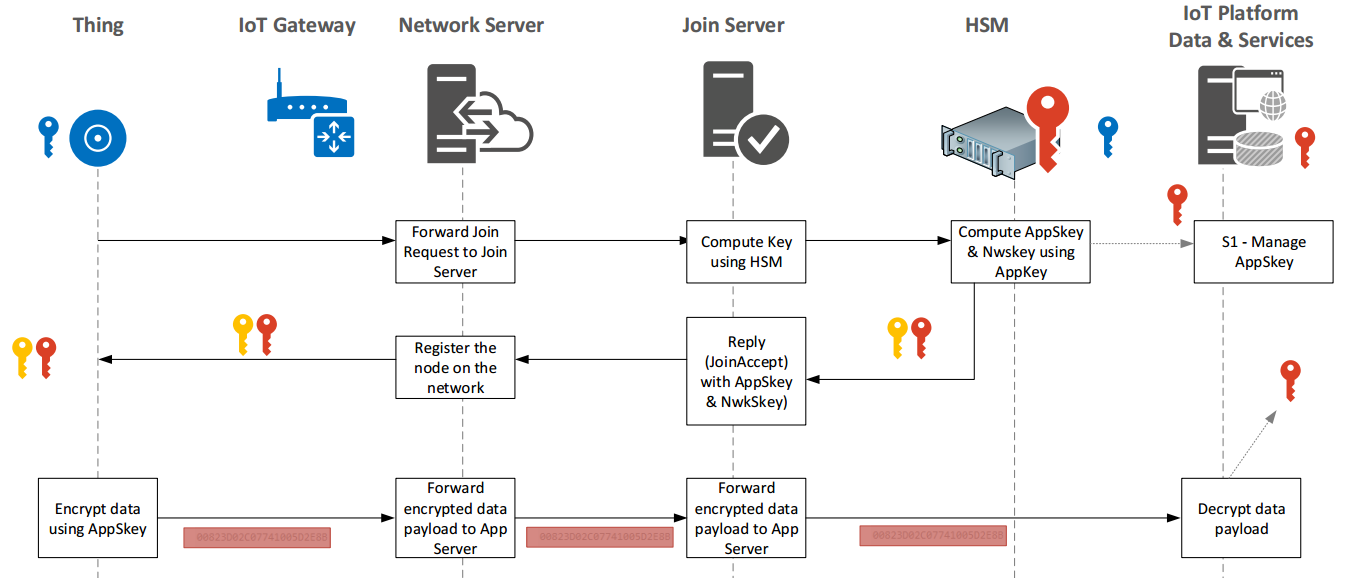
\includegraphics[width=1.0\textwidth]{Figures/Security/smartcanton/smartcanton_joinserver_decrypt_fiware.png}
    \caption{Déchiffrement des données par la plateforme IoT (FIWARE)}
    \label{fig-smartcanton_joinserver_decrypt_fiware}
\end{figure}


La \cref{fig-payload_journey} expose le cheminement complet d'un paquet de données produit par un périphérique (\textit{Thing}) jusqu'à l'application. On peut ainsi voir la répartition des différentes clés sur le schéma. La clé AppKey, la plus importante dans les connexions OTAA, est stockée en sécurité dans le HSM. La seule autre copie de cette clé est sur le périphérique. Le \textit{Network Server} de l'opérateur n'a accès qu'à la Network Session Key, il ne peut ainsi jamais déchiffrer les paquets de données. Cette implémentation reflète le principe qui est conseillé dans les recommandations énoncées à la \cref{sec-security_lorawan_recommendatiions}.

\begin{figure}[ht!]
    \centering
    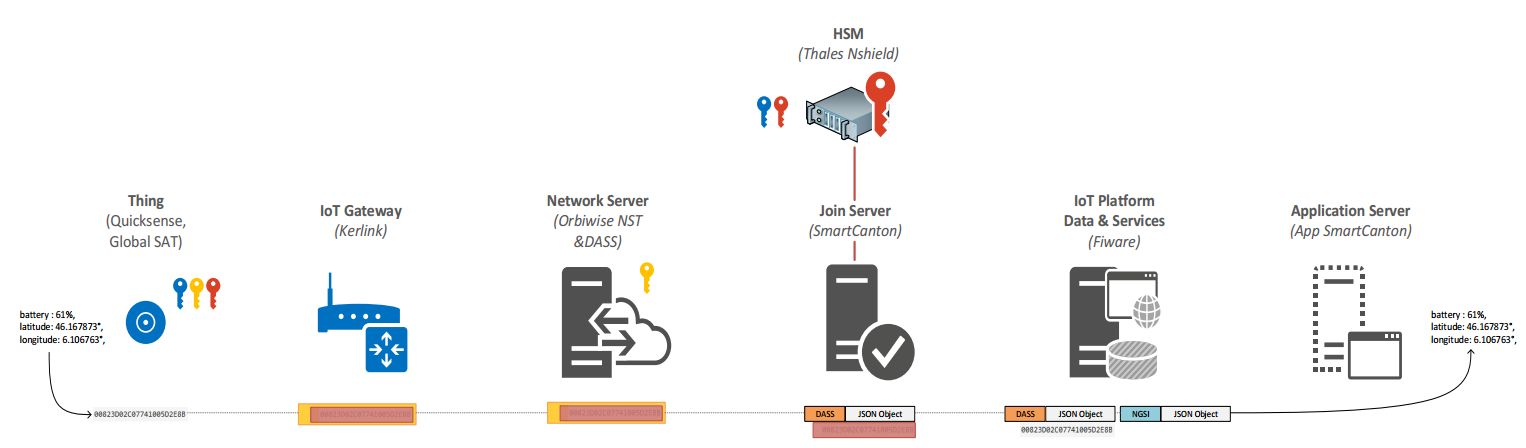
\includegraphics[width=1.0\textwidth]{Figures/Security/smartcanton/payload_journey.png}
    \caption{Cheminement des données depuis le périphérique jusqu'à l'application en utilisant le HSM pour le déchiffrement}
    \label{fig-payload_journey}
\end{figure}





\section{Serveur Web}

Dans le cadre du présent projet, un serveur web a été créé. S'est posée la question de savoir comment sécuriser l'accès à celui-ci. Ci-dessous, une brève explication des deux mécanismes retenus.

\subsection{HTTPS}

Le protocole \textit{HyperText Transfer Protocol Secure} (HTTPS) consiste, de manière résumée, en l'utilisation de la couche HTTP couplée avec un chiffrement à l'aide de SSL ou TLS \cite{HyperTex87:online}. HTTPS a pour but d'identifier (l'identité) le site web auquel le client accède. Pour cela, un certificat d'authentification doit être émis par une autorité de certification tierce, reconnue comme fiable par le navigateur ou système d'exploitation effectuant la requête. Toutes les données communiquées entre le client et le serveur sont chiffrées à l'aide d'une paire de clé publique et clé privée (chiffrement asymétrique) \cite{HyperTex87:online}.

\subsection{JWT}
\label{sec-security_jwt}

Les \textit{JSON Web Tokens} (JWT) sont définis dans un standard \textit{open source} (RFC 7519\footnote{\url{https://tools.ietf.org/html/rfc7519}} \cite{JSONWebT15:online}. Ils offrent la possibilité d'échanger de l'information de manière sécurisée à l'aide d'un jeton signé. Le processus d'identification est illustré à l'aide de la \cref{fig-jwt_connexion}. Il y a deux étapes : 
\begin{enumerate}
    \item L'utilisateur se connecte à un serveur d'authentification afin de récupérer un JWT. Le processus d'identification n'est pas standardisé, le développeur peut ainsi utiliser une \textit{basic authentification} ou un champ clé/valeur dans une requête POST.
    \item L'utilisateur envoie ce JWT dans chacune de ses requêtes vers le serveur applicatif. \\
\end{enumerate}

\begin{figure}[ht!]
    \centering
    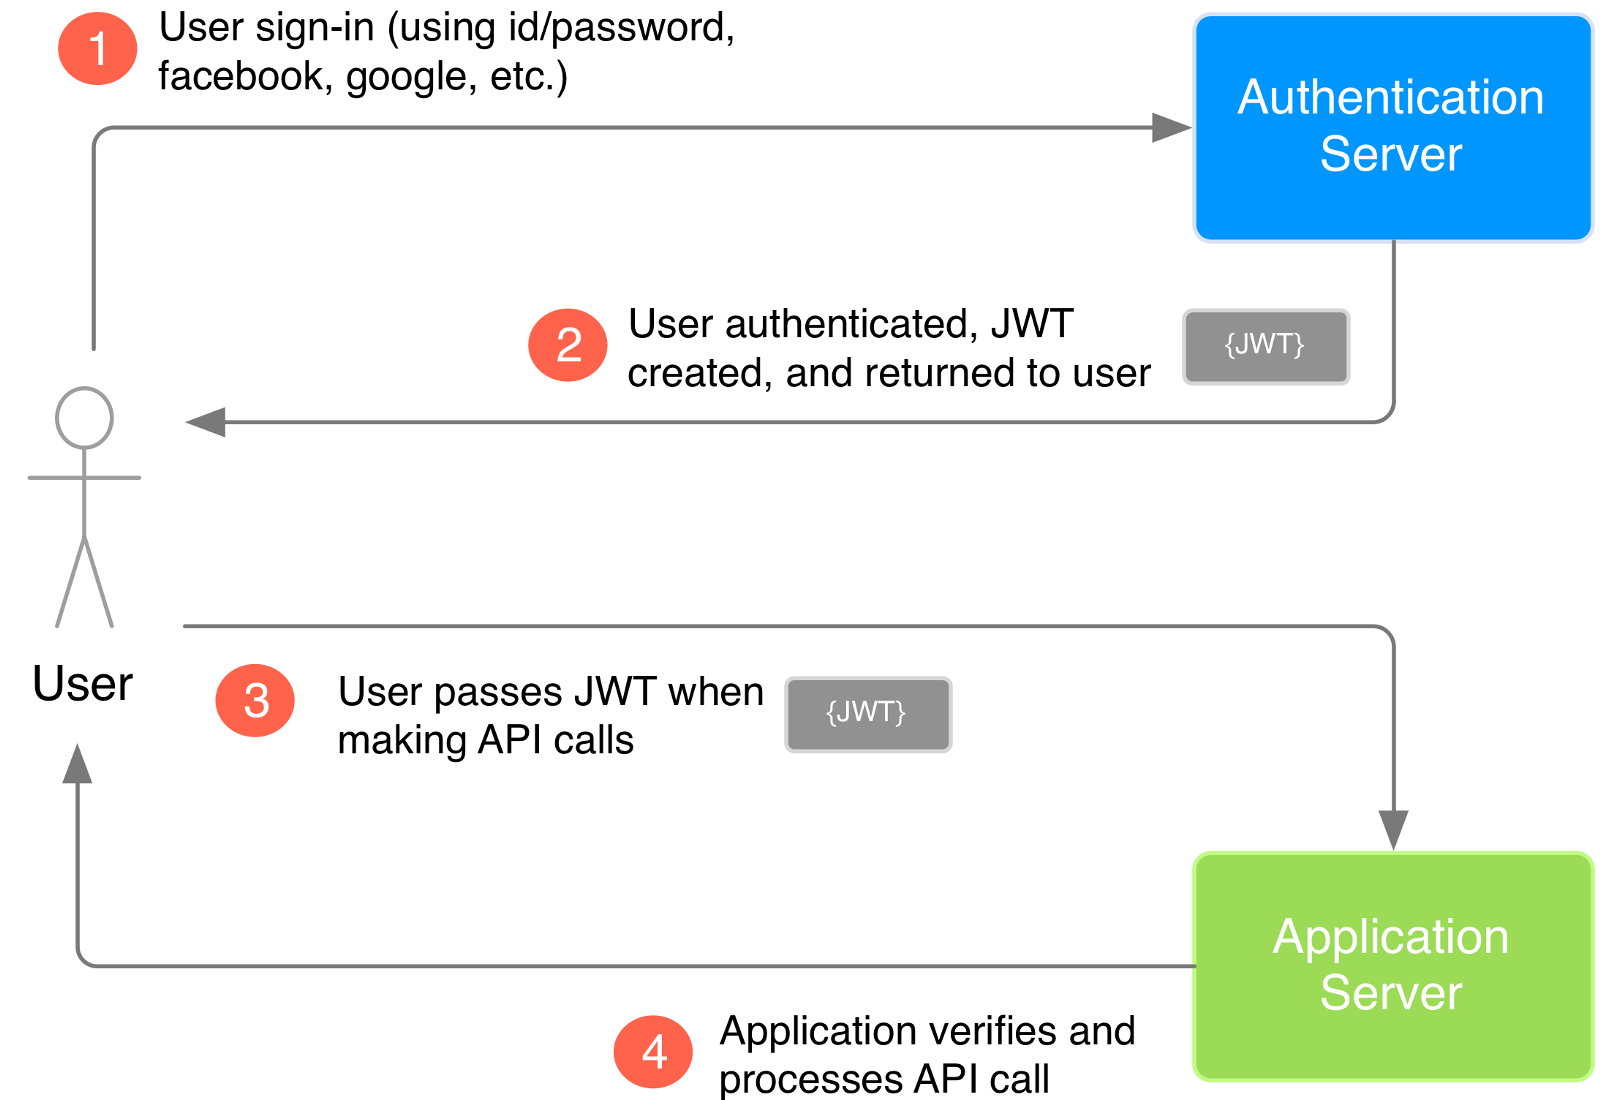
\includegraphics[width=0.8\textwidth]{Figures/Security/jwt_connexion.png}
    \caption{Génération et utilisation d'un \textit{token} JWT}
    \label{fig-jwt_connexion}
\end{figure}

Un JWT est composé de trois champs codés en base64 et séparés par un point. Le site officiel de JWT\footnote{\url{http://jwt.io}} offre la possibilité de déchiffre un \textit{token} directement en ligne. Ce déchiffrement est visible sur la \cref{fig-jwt_token_decrypt} et se décompose comme suit : 
\begin{enumerate}
    \item \textit{Header} : entête contenant uniquement le nom de l'algorithme utilisé pour générer la signature du paquet ainsi que le format du \textit{token}. 
    \item \textit{Payload} : champ modifiable par l'utilisateur comme il le souhaite. Il y a toutefois des clés qui sont standardisées par la norme RFC 7519. Par exemple, la clé \texttt{exp} signifie \textit{Expiration Time} exprimée en heure POSIX\footnote{\url{https://en.wikipedia.org/wiki/Unix_time}}.
    \item \textit{Signature} : champ dérivé de la concaténation des deux champs précédents en base64, sur lequel un chiffrement est appliqué à l'aide de la clé privée basée sur l'algorithme spécifié dans le champ \texttt{Header}. Quand le serveur reçoit un JWT, ce champ est utilisé pour confirmer que le \textit{token} n'a pas été forgé. La clé privée ne quitte jamais le serveur et doit être gardée en lieu sûr.
\end{enumerate}

\begin{figure}[ht!]
    \centering
    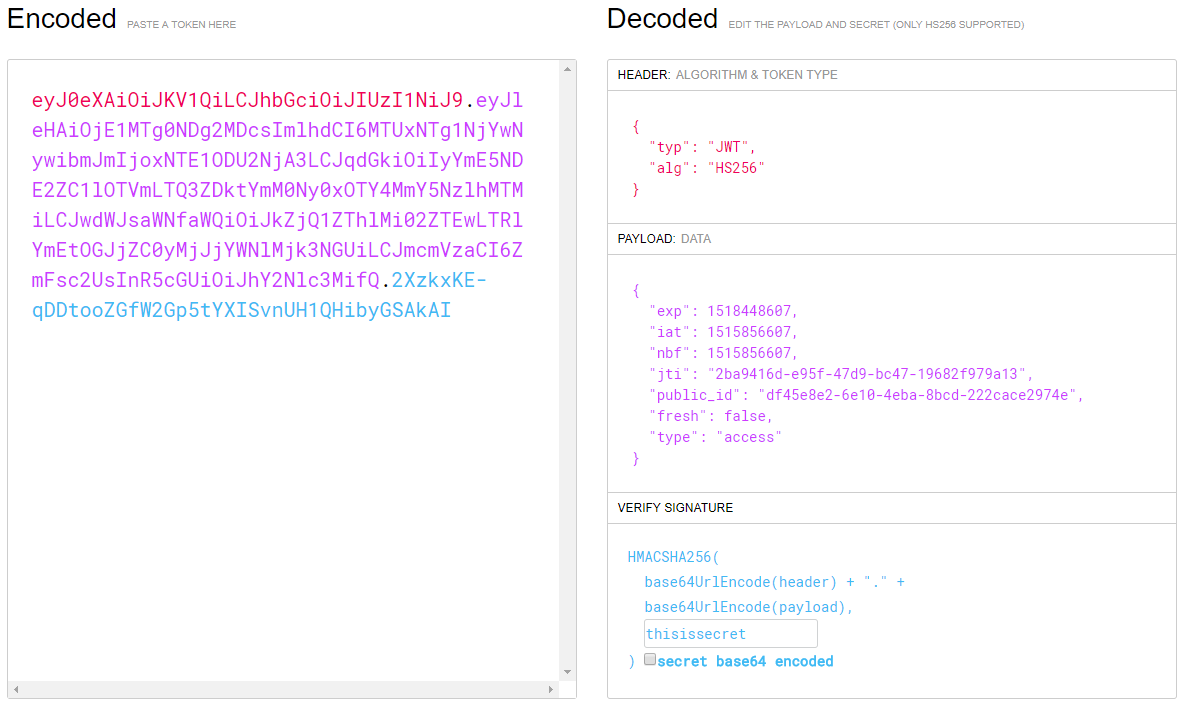
\includegraphics[width=1.0\textwidth]{Figures/Security/jwt_token_decrypt.png}
    \caption{Déchiffrement d'un JWT}
    \label{fig-jwt_token_decrypt}
\end{figure}

Il faut être conscient que les \textit{tokens} JWT n'ajoutent aucune couche de sécurité sur les données. Cela permet d'authentifier l'utilisateur à l'aide d'un \textit{token} temporaire. Cela évite d'envoyer en permanence son \textit{login} et mot de passe dans chacune de ses requêtes. Le développeur peut ainsi gérer automatiquement le concept de sessions et, s’il le souhaite, invalider des \textit{tokens} sans demander à l'utilisateur de changer son mot de passe. Si une personne malveillante s'approprie ce \textit{token}, il pourra toujours l'utiliser pour forcer ses propres requêtes. Pour éviter cela, il convient d'utiliser un protocole qui encapsule les trames avec une couche de sécurité, telle que HTTPS.



\section{Protections matérielles}
\label{sec-security_hardware_protections}

La sécurité est d'autant plus importante lorsqu'un produit est commercialisé. La question n'est pas de savoir si le système est infaillible, car chaque système est accessible d'une façon ou d'une autre, ce n'est souvent qu'une question de temps et de détermination. La réelle question est de savoir quels sont les dangers une fois qu'une personne malveillante a accès à un périphérique et quelles sont les meilleures protections disponibles contre les risques engendrés par ces attaques. Il y a toutefois des mécanismes très simples et peu couteux qui peuvent rendre le travail de personnes malveillantes beaucoup plus difficile. 


\subsection{Détection d'ouverture de boitier}

Il est possible de détecter si un périphérique a été ouvert par une personne, par exemple avec le placement d'un capteur de luminosité à l'intérieur d'un boitier ou de tout autre mécanisme de détection de mouvement. On peut imaginer envoyer un message à la centrale pour notifier un problème et demander à une personne physique de se déplacer pour analyser l'état de la situation. Outrepasser ce mécanisme est néanmoins très simple; il est par exemple possible de se placer dans un milieu qui empêche l'accès au réseau de communications (ex. cage de faraday ou autre). Ce type de mécanismes sont toutefois inutiles si la batterie du dispositif est vide, car les capteurs ne peuvent rien détecter. Il faut ainsi éviter de stocker des informations critiques dans des mémoires non volatiles mal protégées.

\subsection{Protection de la mémoire flash}

Beaucoup de microcontrôleurs proposent des options pour verrouiller les accès à la mémoire flash bloquant ainsi la possibilité de relire le code et de le décompiler pour tenter de trouver des failles dans les implémentations. Le KW41Z de NXP propose ce mode de sécurité. Celui-ci est décrit dans la note d'application AN4507 intitulée \textit{Using the Kinetis Security and Flash Protection Features}\footnote{\url{https://www.nxp.com/docs/en/application-note/AN4507.pdf}}. Voici quelques exemples d'options qui peuvent être activées pour protéger la mémoire flash : 
\begin{enumerate}
    \item \textit{Flash Security} (SEC) : ce mode par défaut est désactivé. La mémoire peut donc être lue et écrite à volonté.
    \item \textit{Mass Erase Enable} (MEEN) : cela permet d'empêcher que le dispositif ne soit reprogrammable à l'aide d'une nouvelle application.
    \item \textit{Freescale Failure Analysis Code} (FSLACC) : ce mode est désactivé par défaut. S’il est activé et que le microcontrôleur est retourné à l'usine de Freescale à cause d'un problème lié à la construction du microcontrôleur, Freescale aura la possibilité d'accéder au contenu de la Flash, et ce, même si la sécurité est activée. La note d'application de Freescale ne fournit pas d'informations supplémentaires sur ce mode.
    \item \textit{Backdoor Key Security} : si l'application a besoin d'écrire dans la mémoire flash, il est possible de forcer la création d'une \textit{backdoor key} offrant la possibilité de désactiver temporairement la sécurité de la mémoire. Ce type d'accès est nécessaire, par exemple, lorsque le microcontrôleur doit mettre à jour son \textit{firmware}. Lorsque le microcontrôleur active cette option, une clé est générée et celle-ci doit être sauvegardée à l'extérieur du microcontrôleur. Lorsque la sécurité devra être désactivée, cette clé sera demandée à l'utilisateur qui devra la fournir à l'aide d'une interface de communication (UART, SPI, I2C, etc.).
\end{enumerate}

Selon le type de sécurité choisie, le JTAG reste accessible, mais uniquement les registres qui lui sont propres en revanche. Si la lecture de la mémoire flash est désactivée, le JTAG ne pourra pas y avoir accès.


\subsection{Coffres-forts matériels}
\label{sec-mcu_stsafe}

Le CMWX1ZZABZ de Murata dispose d'un coffre fort matériel (cf. \cref{sec-hardware_lora_module}) pouvant stocker des informations et être utilisé comme coprocesseur cryptographie. Ce circuit intégré est nommé \textit{STSAFE-A100.} 

Voici une liste des quelques fonctionnalités mises en avant par le fabricant\footnote{\url{http://www.st.com/en/secure-mcus/stsafe-a100.html}} : 
\begin{itemize}
    \item Service de vérification de signature avec possibilité de contrôler un \textit{secure boot} et mise à jour du firmware signée.
    \item Cryptographie asymétrique avancée :
        \begin{itemize}
            \item \textit{Elliptic curve cryptography} (ECC) avec NIST ou Brainpool 256-bit et 384-bit. \textit{curves};
            
            \item \textit{Elliptic curve digital signature algorithm} (ECDSA) avec SHA-256 et SHA-384 pour la génération et vérification de signatures numériques;
            
            \item \textit{Elliptic curve Diffie-Hellman} (ECDH) pour l'établissement des clés.
        \end{itemize}
    \item Cryptographie symétrique avancée :
    \begin{itemize}
        \item \textit{Key wrapping} et \textit{unwrapping} en utilisant AES-128/AES-256;
        
        \item Création de canaux sécurisés basés sur AES-128.
    \end{itemize}
    
    \item Système d'exploitation sécurisé avec protection contre les attaques logicielles et physiques.
\end{itemize}

\begin{figure}[ht!]
    \centering
    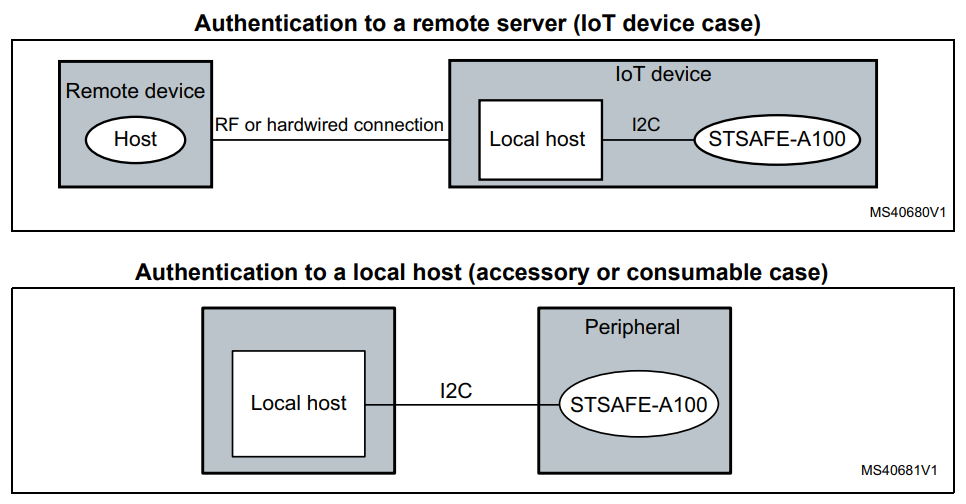
\includegraphics[width=0.7\textwidth]{Figures/Security/stsafe_authentification.png}
    \caption{Authentifications possibles avec un STSAFE}
    \label{fig-stsafe_authentification}
\end{figure}

La communication avec ce module s'effectue à l'aide d'une interface I2C.
Malheureusement, la documentation de ce coffre n'est pas disponible en ligne, à l'exception d'un \textit{databrief}\footnote{\url{http://www.st.com/resource/en/data_brief/stsafe-a100.pdf}} de 15 pages expliquant les caractéristiques principales du circuit et les descriptions matérielles du boitier électronique. Il faut directement s'adresser à STMicroelectronics pour recevoir informations précises sur le module et la programmation (registres I2C). Les fonctionnalités listées par le fabricant demeurent toutefois vagues et, à défaut de documentation, il est difficile d'en apprendre davantage. Cette même \textit{databrief}, présente le schéma illustré en \cref{fig-stsafe_authentification} afin d'expliquer les deux types d'authentification pouvant être utilisé avec ce module. On constate ainsi que ce module peut également authentifier une connexion externe sans fil. Celui-ci peut, par exemple, être couplé à du Bluetooth pour garantir l'identité du maitre initiant la communication sans utiliser de \textit{passkey}. Dans le cadre du présent projet, la première option de ce schéma qui est celle qui présente un réel intérêt.





% \section{IEEE 802.15.4 et les protocoles dérivés}

% Étant donné que le microcontrôleur choisi supporte le standard IEEE 802.15.4, il est intéressant de faire une petit analyse sur la sécurité implémentée dans ce standard. 

% Le standard IEEE 802.15.4 décrit des procédures de sécurité. Le standard décrit quel algorithme de cryptage doit être utilisé pour chiffrer les données à transmettre \cite{Security81:online}. Cependant, le standard ne spécifie pas comment les clés doivent être échangées ni l'authentification de celles-ci. Le standard laisse cela aux couches supérieures. Le protocole ZigBee, qui est le protocole le plus répandu basé sur le standard IEEE 802.15.2.


% IEEE 802.15.4 sets the encryption algorithm to use when cyphering the data to transmit, however,  the standard does not specify how the keys have to be managed or what kind of authentication policies have to be applied. These issues are treated ihttps://www.sharelatex.com/project/595651688581f1b870a4ac64n the upper layers which are managed by technologies such as ZigBee